% Options for packages loaded elsewhere
\PassOptionsToPackage{unicode}{hyperref}
\PassOptionsToPackage{hyphens}{url}
\PassOptionsToPackage{dvipsnames,svgnames,x11names}{xcolor}
%
\documentclass[
  11pt,
]{krantz}
\usepackage{amsmath,amssymb}
\usepackage{lmodern}
\usepackage{iftex}
\ifPDFTeX
  \usepackage[T1]{fontenc}
  \usepackage[utf8]{inputenc}
  \usepackage{textcomp} % provide euro and other symbols
\else % if luatex or xetex
  \usepackage{unicode-math}
  \defaultfontfeatures{Scale=MatchLowercase}
  \defaultfontfeatures[\rmfamily]{Ligatures=TeX,Scale=1}
  \setmonofont[Scale=0.775]{MesloLGS NF}
\fi
% Use upquote if available, for straight quotes in verbatim environments
\IfFileExists{upquote.sty}{\usepackage{upquote}}{}
\IfFileExists{microtype.sty}{% use microtype if available
  \usepackage[]{microtype}
  \UseMicrotypeSet[protrusion]{basicmath} % disable protrusion for tt fonts
}{}
\makeatletter
\@ifundefined{KOMAClassName}{% if non-KOMA class
  \IfFileExists{parskip.sty}{%
    \usepackage{parskip}
  }{% else
    \setlength{\parindent}{0pt}
    \setlength{\parskip}{6pt plus 2pt minus 1pt}}
}{% if KOMA class
  \KOMAoptions{parskip=half}}
\makeatother
\usepackage{xcolor}
\IfFileExists{xurl.sty}{\usepackage{xurl}}{} % add URL line breaks if available
\IfFileExists{bookmark.sty}{\usepackage{bookmark}}{\usepackage{hyperref}}
\hypersetup{
  pdftitle={Data Science per psicologi},
  pdfauthor={Corrado Caudek},
  colorlinks=true,
  linkcolor={Maroon},
  filecolor={Maroon},
  citecolor={Blue},
  urlcolor={Blue},
  pdfcreator={LaTeX via pandoc}}
\urlstyle{same} % disable monospaced font for URLs
\usepackage{color}
\usepackage{fancyvrb}
\newcommand{\VerbBar}{|}
\newcommand{\VERB}{\Verb[commandchars=\\\{\}]}
\DefineVerbatimEnvironment{Highlighting}{Verbatim}{commandchars=\\\{\}}
% Add ',fontsize=\small' for more characters per line
\usepackage{framed}
\definecolor{shadecolor}{RGB}{248,248,248}
\newenvironment{Shaded}{\begin{snugshade}}{\end{snugshade}}
\newcommand{\AlertTok}[1]{\textcolor[rgb]{0.33,0.33,0.33}{#1}}
\newcommand{\AnnotationTok}[1]{\textcolor[rgb]{0.37,0.37,0.37}{\textbf{\textit{#1}}}}
\newcommand{\AttributeTok}[1]{\textcolor[rgb]{0.61,0.61,0.61}{#1}}
\newcommand{\BaseNTok}[1]{\textcolor[rgb]{0.06,0.06,0.06}{#1}}
\newcommand{\BuiltInTok}[1]{#1}
\newcommand{\CharTok}[1]{\textcolor[rgb]{0.5,0.5,0.5}{#1}}
\newcommand{\CommentTok}[1]{\textcolor[rgb]{0.37,0.37,0.37}{\textit{#1}}}
\newcommand{\CommentVarTok}[1]{\textcolor[rgb]{0.37,0.37,0.37}{\textbf{\textit{#1}}}}
\newcommand{\ConstantTok}[1]{\textcolor[rgb]{0,0,0}{#1}}
\newcommand{\ControlFlowTok}[1]{\textcolor[rgb]{0.27,0.27,0.27}{\textbf{#1}}}
\newcommand{\DataTypeTok}[1]{\textcolor[rgb]{0.27,0.27,0.27}{#1}}
\newcommand{\DecValTok}[1]{\textcolor[rgb]{0.06,0.06,0.06}{#1}}
\newcommand{\DocumentationTok}[1]{\textcolor[rgb]{0.37,0.37,0.37}{\textbf{\textit{#1}}}}
\newcommand{\ErrorTok}[1]{\textcolor[rgb]{0.14,0.14,0.14}{\textbf{#1}}}
\newcommand{\ExtensionTok}[1]{#1}
\newcommand{\FloatTok}[1]{\textcolor[rgb]{0.06,0.06,0.06}{#1}}
\newcommand{\FunctionTok}[1]{\textcolor[rgb]{0,0,0}{#1}}
\newcommand{\ImportTok}[1]{#1}
\newcommand{\InformationTok}[1]{\textcolor[rgb]{0.37,0.37,0.37}{\textbf{\textit{#1}}}}
\newcommand{\KeywordTok}[1]{\textcolor[rgb]{0.27,0.27,0.27}{\textbf{#1}}}
\newcommand{\NormalTok}[1]{#1}
\newcommand{\OperatorTok}[1]{\textcolor[rgb]{0.43,0.43,0.43}{\textbf{#1}}}
\newcommand{\OtherTok}[1]{\textcolor[rgb]{0.37,0.37,0.37}{#1}}
\newcommand{\PreprocessorTok}[1]{\textcolor[rgb]{0.37,0.37,0.37}{\textit{#1}}}
\newcommand{\RegionMarkerTok}[1]{#1}
\newcommand{\SpecialCharTok}[1]{\textcolor[rgb]{0,0,0}{#1}}
\newcommand{\SpecialStringTok}[1]{\textcolor[rgb]{0.5,0.5,0.5}{#1}}
\newcommand{\StringTok}[1]{\textcolor[rgb]{0.5,0.5,0.5}{#1}}
\newcommand{\VariableTok}[1]{\textcolor[rgb]{0,0,0}{#1}}
\newcommand{\VerbatimStringTok}[1]{\textcolor[rgb]{0.5,0.5,0.5}{#1}}
\newcommand{\WarningTok}[1]{\textcolor[rgb]{0.37,0.37,0.37}{\textbf{\textit{#1}}}}
\usepackage{longtable,booktabs,array}
\usepackage{calc} % for calculating minipage widths
% Correct order of tables after \paragraph or \subparagraph
\usepackage{etoolbox}
\makeatletter
\patchcmd\longtable{\par}{\if@noskipsec\mbox{}\fi\par}{}{}
\makeatother
% Allow footnotes in longtable head/foot
\IfFileExists{footnotehyper.sty}{\usepackage{footnotehyper}}{\usepackage{footnote}}
\makesavenoteenv{longtable}
\usepackage{graphicx}
\makeatletter
\def\maxwidth{\ifdim\Gin@nat@width>\linewidth\linewidth\else\Gin@nat@width\fi}
\def\maxheight{\ifdim\Gin@nat@height>\textheight\textheight\else\Gin@nat@height\fi}
\makeatother
% Scale images if necessary, so that they will not overflow the page
% margins by default, and it is still possible to overwrite the defaults
% using explicit options in \includegraphics[width, height, ...]{}
\setkeys{Gin}{width=\maxwidth,height=\maxheight,keepaspectratio}
% Set default figure placement to htbp
\makeatletter
\def\fps@figure{htbp}
\makeatother
\setlength{\emergencystretch}{3em} % prevent overfull lines
\providecommand{\tightlist}{%
  \setlength{\itemsep}{0pt}\setlength{\parskip}{0pt}}
\setcounter{secnumdepth}{5}
\usepackage{amsmath}
\usepackage{amssymb}
\usepackage{amsfonts}

\defaultfontfeatures{Scale=MatchLowercase}

\usepackage{booktabs}
\usepackage{longtable}
\usepackage[bf,singlelinecheck=off]{caption}

\usepackage{framed,color}
\definecolor{shadecolor}{RGB}{248,248,248}

\renewcommand{\textfraction}{0.05}
\renewcommand{\topfraction}{0.8}
\renewcommand{\bottomfraction}{0.8}
\renewcommand{\floatpagefraction}{0.75}

\renewenvironment{quote}{\begin{VF}}{\end{VF}}
\let\oldhref\href
\renewcommand{\href}[2]{#2\footnote{\url{#1}}}

\ifxetex
  \usepackage{letltxmacro}
  \setlength{\XeTeXLinkMargin}{1pt}
  \LetLtxMacro\SavedIncludeGraphics\includegraphics
  \def\includegraphics#1#{% #1 catches optional stuff (star/opt. arg.)
    \IncludeGraphicsAux{#1}%
  }%
  \newcommand*{\IncludeGraphicsAux}[2]{%
    \XeTeXLinkBox{%
      \SavedIncludeGraphics#1{#2}%
    }%
  }%
\fi

\makeatletter
\newenvironment{kframe}{%
\medskip{}
\setlength{\fboxsep}{.8em}
 \def\at@end@of@kframe{}%
 \ifinner\ifhmode%
  \def\at@end@of@kframe{\end{minipage}}%
  \begin{minipage}{\columnwidth}%
 \fi\fi%
 \def\FrameCommand##1{\hskip\@totalleftmargin \hskip-\fboxsep
 \colorbox{shadecolor}{##1}\hskip-\fboxsep
     % There is no \\@totalrightmargin, so:
     \hskip-\linewidth \hskip-\@totalleftmargin \hskip\columnwidth}%
 \MakeFramed {\advance\hsize-\width
   \@totalleftmargin\z@ \linewidth\hsize
   \@setminipage}}%
 {\par\unskip\endMakeFramed%
 \at@end@of@kframe}
\makeatother

\renewenvironment{Shaded}{\begin{kframe}}{\end{kframe}}

\usepackage{makeidx}
\makeindex

\urlstyle{tt}

\usepackage{amsthm}
\makeatletter
\def\thm@space@setup{%
  \thm@preskip=8pt plus 2pt minus 4pt
  \thm@postskip=\thm@preskip
}
\makeatother

\DeclareMathOperator{\V}{\mathbb{V}} % Define variance operator
\DeclareMathOperator{\Var}{\mathbb{V}} % Define variance operator
\DeclareMathOperator{\SD}{SD} % Define sd operator
\DeclareMathOperator{\Cov}{Cov} % Define covariance operator
\DeclareMathOperator{\Corr}{Corr} % Define correlation operator
\DeclareMathOperator{\Me}{Me} % Define mediane operator
\DeclareMathOperator{\Mo}{Mo} % Define mode operator

\DeclareMathOperator{\Bin}{Binomial} % Define binomial operator
\DeclareMathOperator{\Bernoulli}{Bernoulli} % Define Bernoulli operator
\DeclareMathOperator{\Ber}{\mathscr{B}} % Define Bernoulli operator
\DeclareMathOperator{\Poi}{Poisson} % Define Poisson operator
\DeclareMathOperator{\Uniform}{Uniform} % Define Uniform operator
\DeclareMathOperator{\Cauchy}{Cauchy} % Define Cauchy operator
\DeclareMathOperator{\B}{B} % beta function
% \mbox{B}(a, b) % beta function
% \mbox{Beta}(a, b) % beta distribution

\DeclareMathOperator{\elpd}{elpd} % Define elpd operator
\DeclareMathOperator{\lppd}{lppd} % Define lppd operator
\DeclareMathOperator{\LOO}{LOO} % Define LOO operator
\DeclareMathOperator{\argmin}{arg\,min} 
\DeclareMathOperator{\argmax}{arg\,max} 

\newcommand{\E}{\mathbb{E}} % Define expected value operator
\newcommand{\R}{\textsf{R}} % Define R programming language symbol
\newcommand{\Real}{\mathbb{R}} % Define real number operator
\newcommand{\Prob}{\mathscr{P}}
\newcommand{\indep}{\perp \!\!\! \perp}

\usepackage[
 labelfont=bf,
 font={small, it}
]{caption}
\usepackage{upquote} % print correct quotes in verbatim-environments
\usepackage{empheq}
\usepackage{xfrac}

\usepackage{polyglossia}
\setmainlanguage{italian}

\frontmatter
\ifLuaTeX
  \usepackage{selnolig}  % disable illegal ligatures
\fi
\usepackage[]{natbib}
\bibliographystyle{apalike}

\title{Data Science per psicologi}
\author{Corrado Caudek}
\date{2022-02-21}

\usepackage{amsthm}
\newtheorem{theorem}{Teorema}[chapter]
\newtheorem{lemma}{Lemma}[chapter]
\newtheorem{corollary}{Corollario}[chapter]
\newtheorem{proposition}{Proposizione}[chapter]
\newtheorem{conjecture}{Congettura}[chapter]
\theoremstyle{definition}
\newtheorem{definition}{Definizione}[chapter]
\theoremstyle{definition}
\newtheorem{example}{Esempio}[chapter]
\theoremstyle{definition}
\newtheorem{exercise}{Esercizio}[chapter]
\theoremstyle{definition}
\newtheorem{hypothesis}{Hypothesis}[chapter]
\theoremstyle{remark}
\newtheorem*{remark}{Osservazione}
\newtheorem*{solution}{Soluzione}
\begin{document}
\maketitle

\cleardoublepage\newpage\thispagestyle{empty}\null
% \cleardoublepage\newpage\thispagestyle{empty}\null
%\cleardoublepage\newpage
\thispagestyle{empty}
\begin{center}
\Large{Psicometria -- AA 2021/2022}

\vskip20pt

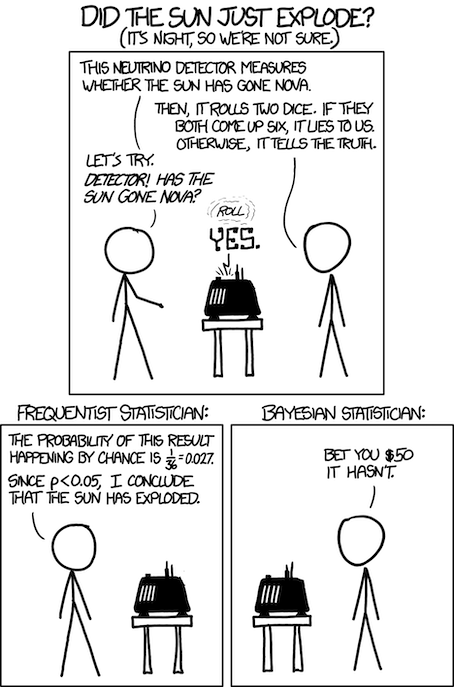
\includegraphics{images/frequentists_vs_bayesians.png}
\end{center}

\setlength{\abovedisplayskip}{-5pt}
\setlength{\abovedisplayshortskip}{-5pt}

{
\hypersetup{linkcolor=}
\setcounter{tocdepth}{2}
\tableofcontents
}
\listoffigures
\listoftables
\hypertarget{prefazione}{%
\chapter*{Prefazione}\label{prefazione}}


\emph{Data Science per psicologi} contiene il materiale delle lezioni dell'insegnamento di \emph{Psicometria B000286} (A.A. 2021/2022) rivolto agli studenti del primo anno del Corso di Laurea in Scienze e Tecniche Psicologiche dell'Università degli Studi di Firenze. \emph{Psicometria} si propone di fornire agli studenti un'introduzione all'analisi dei dati in psicologia. Le conoscenze/competenze che verranno sviluppate in questo insegnamento sono quelle della Data science, ovvero un insieme di conoscenze/competenze che si pongono all'intersezione tra statistica (ovvero, richiedono la capacità di comprendere teoremi statistici) e informatica (ovvero, richiedono la capacità di sapere utilizzare un software).

\hypertarget{la-psicologia-e-la-data-science}{%
\section*{La psicologia e la Data science}\label{la-psicologia-e-la-data-science}}


Sembra sensato spendere due parole su un tema che è importante per gli studenti: quello indicato dal titolo di questo Capitolo. È ovvio che agli studenti di psicologia la statistica non piace. Se piacesse, forse studierebbero Data science e non psicologia; ma non lo fanno. Di conseguenza, gli studenti di psicologia si chiedono: ``perché dobbiamo perdere tanto tempo a studiare queste cose quando in realtà quello che ci interessa è tutt'altro?'' Questa è una bella domanda.

C'è una ragione molto semplice che dovrebbe farci capire perché la Data science è così importante per la psicologia. Infatti, a ben pensarci, la psicologia è una disciplina intrinsecamente statistica, se per statistica intendiamo quella disciplina che studia la variazione delle caratteristiche degli individui nella popolazione. La psicologia studia \emph{gli individui} ed è proprio la variabilità inter- e intra-individuale ciò che vogliamo descrivere e, in certi casi, predire. In questo senso, la psicologia è molto diversa dall'ingegneria, per esempio. Le proprietà di un determinato ponte sotto certe condizioni, ad esempio, sono molto simili a quelle di un altro ponte, sotto le medesime condizioni. Quindi, per un ingegnere la statistica è poco importante: le proprietà dei materiali sono unicamente dipendenti dalla loro composizione e restano costanti. Ma lo stesso non può dirsi degli individui: ogni individuo è unico e cambia nel tempo. E le variazioni tra gli individui, e di un individuo nel tempo, sono l'oggetto di studio proprio della psicologia: è dunque chiaro che i problemi che la psicologia si pone sono molto diversi da quelli affrontati, per esempio, dagli ingegneri. Questa è la ragione per cui abbiamo tanto bisogno della Data science in psicologia: perché la Data science ci consente di descrivere la variazione e il cambiamento. E queste sono appunto le caratteristiche di base dei fenomeni psicologici.

Sono sicuro che, leggendo queste righe, a molti studenti sarà venuta in mente la seguente domanda: perché non chiediamo a qualche esperto di fare il ``lavoro sporco'' (ovvero le analisi statistiche) per noi, mentre noi (gli psicologi) ci occupiamo solo di ciò che ci interessa, ovvero dei problemi psicologici slegati dai dettagli ``tecnici'' della Data science? La risposta a questa domanda è che non è possibile progettare uno studio psicologico sensato senza avere almeno una comprensione rudimentale della Data science. Le tematiche della Data science non possono essere ignorate né dai ricercatori in psicologia né da coloro che svolgono la professione di psicologo al di fuori dell'Università. Infatti, anche i professionisti al di fuori dall'università non possono fare a meno di leggere la letteratura psicologica più recente: il continuo aggiornamento delle conoscenze è infatti richiesto dalla deontologia della professione. Ma per potere fare questo è necessario conoscere un bel po' di Data science! Basta aprire a caso una rivista specialistica di psicologia per rendersi conto di quanto ciò sia vero: gli articoli che riportano i risultati delle ricerche psicologiche sono zeppi di analisi statistiche e di modelli formali. E la comprensione della letteratura psicologica rappresenta un requisito minimo nel bagaglio professionale dello psicologo.

Le considerazioni precedenti cercano di chiarire il seguente punto: la Data science non è qualcosa da studiare a malincuore, in un singolo insegnamento universitario, per poi poterla tranquillamente dimenticare. Nel bene e nel male, gli psicologi usano gli strumenti della Data science in tantissimi ambiti della loro attività professionale: in particolare quando costruiscono, somministrano e interpretano i test psicometrici. È dunque chiaro che possedere delle solide basi di Data science è un tassello imprescindibile del bagaglio professionale dello psicologo. In questo insegnamento verrano trattati i temi base della Data science e verrà adottato un punto di vista bayesiano, che corrisponde all'approccio più recente e sempre più diffuso in psicologia.

\hypertarget{come-studiare}{%
\section*{Come studiare}\label{come-studiare}}


Il giusto metodo di studio per prepararsi all'esame di Psicometria è quello di seguire attivamente le lezioni, assimilare i concetti via via che essi vengono presentati e verificare in autonomia le procedure presentate a lezione. Incoraggio gli studenti a farmi domande per chiarire ciò che non è stato capito appieno. Incoraggio gli studenti a utilizzare i forum attivi su Moodle e, soprattutto, a svolgere gli esercizi proposti su Moodle. I problemi forniti su Moodle rappresentano il livello di difficoltà richiesto per superare l'esame e consentono allo studente di comprendere se le competenze sviluppate fino a quel punto sono sufficienti rispetto alle richieste dell'esame.

La prima fase dello studio, che è sicuramente individuale, è quella in cui è necessario acquisire le conoscenze teoriche relative ai problemi che saranno presentati all'esame. La seconda fase di studio, che può essere facilitata da scambi con altri e da incontri di gruppo, porta ad acquisire la capacità di applicare le conoscenze: è necessario capire come usare un software (\(\textsf{R}\)) per applicare i concetti statistici alla specifica situazione del problema che si vuole risolvere. Le due fasi non sono però separate: il saper fare molto spesso ci aiuta a capire meglio.

\hypertarget{sviluppare-un-metodo-di-studio-efficace}{%
\section*{Sviluppare un metodo di studio efficace}\label{sviluppare-un-metodo-di-studio-efficace}}


Avendo insegnato molte volte in passato un corso introduttivo di analisi dei dati ho notato nel corso degli anni che gli studenti con l'atteggiamento mentale che descriverò qui sotto generalmente ottengono ottimi risultati. Alcuni studenti sviluppano naturalmente questo approccio allo studio, ma altri hanno bisogno di fare uno sforzo per maturarlo. Fornisco qui sotto una breve descrizione del ``metodo di studio'' che, nella mia esperienza, è il più efficace per affrontare le richieste di questo insegnamento.

\begin{itemize}
\tightlist
\item
  Dedicate un tempo sufficiente al materiale di base, apparentemente facile; assicuratevi di averlo capito bene. Cercate le lacune nella vostra comprensione. Leggere presentazioni diverse dello stesso materiale (in libri o articoli diversi) può fornire nuove intuizioni.
\item
  Gli errori che facciamo sono i nostri migliori maestri. Istintivamente cerchiamo di dimenticare subito i nostri errori. Ma il miglior modo di imparare è apprendere dagli errori che commettiamo. In questo senso, una soluzione corretta è meno utile di una soluzione sbagliata. Quando commettiamo un errore questo ci fornisce un'informazione importante: ci fa capire qual è il materiale di studio sul quale dobbiamo ritornare e che dobbiamo capire meglio.
\item
  C'è ovviamente un aspetto ``psicologico'' nello studio. Quando un esercizio o problema ci sembra incomprensibile, la cosa migliore da fare è dire: ``mi arrendo'', ``non ho idea di cosa fare!''. Questo ci rilassa: ci siamo già arresi, quindi non abbiamo niente da perdere, non dobbiamo più preoccuparci. Ma non dobbiamo fermarci qui. Le cose ``migliori'' che faccio (se ci sono) le faccio quando non ho voglia di lavorare. Alle volte, quando c'è qualcosa che non so fare e non ho idea di come affontare, mi dico: ``oggi non ho proprio voglia di fare fatica'', non ho voglia di mettermi nello stato mentale per cui ``in 10 minuti devo risolvere il problema perché dopo devo fare altre cose''. Però ho voglia di \emph{divertirmi} con quel problema e allora mi dedico a qualche aspetto ``marginale'' del problema, che so come affrontare, oppure considero l'aspetto più difficile del problema, quello che non so come risolvere, ma invece di cercare di risolverlo, guardo come altre persone hanno affrontato problemi simili, opppure lo stesso problema in un altro contesto. Non mi pongo l'obiettivo ``risolvi il problema in 10 minuti'', ma invece quello di farmi un'idea ``generale'' del problema, o quello di capire un caso più specifico e più semplice del problema. Senza nessuna pressione. Infatti, in quel momento ho deciso di non lavorare (ovvero, di non fare fatica). Va benissimo se ``parto per la tangente'', ovvero se mi metto a leggere del materiale che sembra avere poco a che fare con il problema centrale (le nostre intuizioni e la nostra curiosità solitamente ci indirizzano sulla strada giusta). Quando faccio così, molto spesso trovo la soluzione del problema che mi ero posto e, paradossalmente, la trovo in un tempo minore di quello che, in precedenza, avevo dedicato a ``lavorare'' al problema. Allora perché non faccio sempre così? C'è ovviamente l'aspetto dei ``10 minuti'' che non è sempre facile da dimenticare. Sotto pressione, possiamo solo agire in maniera automatica, ovvero possiamo solo applicare qualcosa che già sappiamo fare. Ma se dobbiamo imparare qualcosa di nuovo, la pressione è un impedimento.
\item
  È utile farsi da soli delle domande sugli argomenti trattati, senza limitarsi a cercare di risolvere gli esercizi che vengono assegnati. Quando studio qualcosa mi viene in mente: ``se questo è vero, allora deve succedere quest'altra cosa''. Allora verifico se questo è vero, di solito con una simulazione. Se i risultati della simulazione sono quelli che mi aspetto, allora vuol dire che ho capito. Se i risultati sono diversi da quelli che mi aspettavo, allora mi rendo conto di non avere capito e ritorno indietro a studiare con più attenzione la teoria che pensavo di avere capito -- e ovviamente mi rendo conto che c'era un aspetto che avevo frainteso. Questo tipo di verifica è qualcosa che dobbiamo fare da soli, in prima persona: nessun altro può fare questo al posto nostro.
\item
  Non aspettatevi di capire tutto la prima volta che incontrate un argomento nuovo.\footnote{Ricordatevi inoltre che gli individui tendono a sottostimare la propria capacità di apprendere \citep{horn2021underestimating}.} È utile farsi una nota mentalmente delle lacune nella vostra comprensione e tornare su di esse in seguito per carcare di colmarle. L'atteggiamento naturale, quando non capiamo i dettagli di qualcosa, è quello di pensare: ``non importa, ho capito in maniera approssimativa questo punto, non devo preoccuparmi del resto''. Ma in realtà non è vero: se la nostra comprensione è superficiale, quando il problema verrà presentato in una nuova forma, non riusciremo a risolverlo. Per cui i dubbi che ci vengono quando studiamo qualcosa sono il nostro alleato più prezioso: ci dicono esattamente quali sono gli aspetti che dobbiamo approfondire per potere migliorare la nostra preparazione.
\item
  È utile sviluppare una visione d'insieme degli argomenti trattati, capire l'obiettivo generale che si vuole raggiungere e avere chiaro il contributo che i vari pezzi di informazione forniscono al raggiungimento di tale obiettivo. Questa organizzazione mentale del materiale di studio facilita la comprensione. È estremamente utile creare degli schemi di ciò che si sta studiando. Non aspettate che sia io a fornirvi un riepilogo di ciò che dovete imparare: sviluppate da soli tali schemi e tali riassunti.
\item
  Tutti noi dobbiamo imparare l'arte di trovare le informazioni, non solo nel caso di questo insegnamento. Quando vi trovate di fronte a qualcosa che non capite, o ottenete un oscuro messaggio di errore da un software, ricordatevi: ``Google is your friend''!
\end{itemize}

\begin{flushright}
Corrado Caudek\\
Marzo 2022 \end{flushright}

\mainmatter

\hypertarget{part-il-calcolo-delle-probabilituxe0}{%
\part{Il calcolo delle probabilità}\label{part-il-calcolo-delle-probabilituxe0}}

\hypertarget{intro-prob-1}{%
\chapter{La logica dell'incerto}\label{intro-prob-1}}

In questa parte della dispensa verrà introdotta la teoria delle probabilità. Prima di entrare nei dettagli, cerchiamo di capire perché la probabilità sia cruciale per la ricerca scientifica.

La teoria delle probabilità è cruciale per la scienza perché la ricerca procede mediante l'inferenza induttiva. Non siamo mai completamente sicuri della verità di una proposizione (ipotesi, teoria): al valore di verità di una proposizione possiamo solo assegnare un giudizio probabilistico. L'approccio bayesiano è una scuola di pensiero che usa la probabilità per quantificare il grado di fiducia che può essere attribuito ad una proposizione. L'inferenza statistica bayesiana è un tipo di inferenza induttiva che ha lo scopo di quantificare la fiducia che si ha nell'ipotesi \(H\) dopo il verificarsi del dato d'evidenza \(E\). Per quantificare un tale grado di fiducia l'inferenza statistica bayesiana utilizza la teoria delle probabilità. Una comprensione dell'inferenza statistica bayesiana richiede dunque, preliminarmente, la conoscenze della teoria delle probabilità.

\hypertarget{che-cosuxe8-la-probabilituxe0}{%
\section{Che cos'è la probabilità?}\label{che-cosuxe8-la-probabilituxe0}}

La definizione della probabilità è un problema estremamente dibattuto ed aperto. Sono state fornite due possibili soluzioni al problema di definire il concetto di probabilità.

\begin{enumerate}
\def\labelenumi{(\alph{enumi})}
\item
  La natura della probabilità è ``ontologica'' (ovvero, basata sulla metafisica): la probabilità è una proprietà della della realtà, del mondo, di come sono le cose, indipendentemente dalla nostra esperienza. È una visione che qualcuno chiama ``oggettiva''.
\item
  La natura della probabilità è ``epistemica'' (ovvero, basata sulla conoscenza): la probabilità si riferisce alla conoscenza che abbiamo del mondo, non al mondo in sé. Di conseguenza è detta, in contrapposizione alla precedente definizione, ``soggettiva''.
\end{enumerate}

In termini epistemici, la probabilità fornisce una misura della nostra incertezza sul verificarsi di un fenomeno, alla luce delle informazioni disponibili. Potremmo dire che c'è una ``scala'' naturale che ha per estremi il vero (1: evento certo) da una parte ed il falso (0: evento impossibile) dall'altra. La probabilità è la quantificazione di questa scala: descrive lo stato della nostra incertezza rispetto al contenuto di verità di una proposizione.

Nell'interpretazione frequentista, la probabilità \(P(E)\) rappresenta la frequenza relativa a lungo termine di un grande numero di ripetizioni di un esperimento casuale sotto le medesime condizioni. Viene stressata qui l'idea che ciò di cui parliamo è qualcosa che emerge nel momento in cui è possibile ripetere l'esperimento casuale tante volte sotto le medesime condizioni -- sono invece esclusi gli eventi unici e irripetibili.

L'interpretazione bayesiana della probabilità fa invece ricorso ad una concezione più ampia, non legata al solo evento in sé ma che include anche il soggetto assegnante la funzione di probabilità. In pratica l'assegnazione di probabilità bayesiana viene effettuata dal decisore, in base alle proprie conoscenze a priori integrate con tutto il generico bagaglio culturale personale. In questo modo, la probabilità non sarà obbligatoriamente la stessa per tutti i soggetti, ma variarierà a seconda delle informazioni a disposizione, dell'esperienza personale e soprattutto del punto di vista proprio di ogni decisore ed è dunque assimilabile al ``grado di fiducia'' -- in inglese \emph{degree of belief} -- di un dato soggetto, in un dato istante e con un dato insieme d'informazioni, circa l'accadere dell'evento \(E\). ``{[}N{]}essuna scienza ci permetterà di dire: il tale fatto accadrà, andrà così e così, perché ciò è conseguenza di tale legge, e tale legge è una verità assoluta, ma tanto meno ci condurrà a concludere scetticamente: la verità assoluta non esiste, e quindi tale fatto può accadere e può non accadere, può andare così e può andare in tutt'altro modo, nulla io ne so. Quel che si potrà dire è questo: io prevedo che il tale fatto avverrà, e avverrà nel tal modo, perché l'esperienza del passato e l'elaborazione scientifica cui il pensiero dell'uomo l'ha sottoposta mi fanno sembrare ragionevole questa previsione'' \citep{definetti1931prob}.

L'impostazione bayesiana, sviluppata da Ramsey e de Finetti, riconduce l'assegnazione di probabilità allo scommettere sul verificarsi di un evento: la probabilità di un evento \(E\) è la quota \(p(E)\) che un individuo reputa di dover pagare ad un banco per ricevere ``1'' ovvero ``0'' verificandosi o non verificandosi \(E\).

Secondo De Finetti, le valutazioni di probabilità degli eventi devono rispondere ai principi di equità e coerenza. Una scommessa risponde al principio di \emph{equità} se il ruolo di banco e giocatore sono scambiabili in ogni momento del gioco e sempre alle stesse condizioni. Una scommessa risponde al principio di \emph{coerenza} se non vi sono combinazioni di scommesse che consentano (sia al banco che al giocatore) di realizzare perdite o vincite certe.

L'approccio definettiano dell'impostazione della scommessa si basa dunque sulle assunzioni di razionalità e coerenza del decisore, al quale è fatto esplicito divieto di effettuare scommesse a perdita o guadagno certo. Il decisore, proponendo la scommessa, deve essere disposto a scambiare il posto dello scommettitore con quello del banco.

Il metodo della scommessa, oltre che una definizione, fornisce un mezzo operativo di assegnazione della probabilità. Sulla base di questa definizione operativa, che si può ritenere ragionevolmente soddisfatta dal comportamento di un qualunque individuo che agisca in modo razionale in condizioni di incertezza, possono essere agevolmente dimostrate tutte le proprietà classiche della probabilità: essa non può assumere valori negativi, né può essere superiore all'unità; se \(E\) è un evento certo, la sua probabilità è 1; se invece \(E\) è un evento impossibile, la sua probabilità è 0.

I problemi posti dall'approccio definettiano riguardano l'arbitrarietà dell'assegnazione soggettività di probabilità la quale sembra negare la validità dell'intero costrutto teorico. In risposta a tale critica, i bayesiani sostengono che gli approcci oggettivisti alla probabilità nascondono scelte arbitrarie preliminari e sono basate su assunzioni implausibili. È molto più onesto esplicitare subito tutte le scelte arbitrarie effettuate nel corso dell'analisi in modo da controllarne coerenza e razionalità.

\hypertarget{variabili-casuali-e-probabilituxe0-di-un-evento}{%
\section{Variabili casuali e probabilità di un evento}\label{variabili-casuali-e-probabilituxe0-di-un-evento}}

Esaminiamo qui di seguito alcuni concetti di base della teoria delle probabilità.

\hypertarget{eventi-e-probabilituxe0}{%
\subsection{Eventi e probabilità}\label{eventi-e-probabilituxe0}}

Nella teoria delle probabilità il risultato ``testa'' nel lancio di una moneta è chiamato \emph{evento}.\footnote{Per un ripasso delle nozioni di base della teoria degli insiemi, si veda l'Appendice \ref{insiemistica}.} Ad esempio, \(Y\) = 1 denota l'evento in cui il lancio di una moneta produce come risultato testa. Il funzionale \(P(·)\) definisce la probabilità di un evento. Ad esempio, per il lancio di una moneta equilibrata, la probabilità dell'evento ``il risultato del lancio della moneta è testa'' è scritta come \(P(Y = 1) = 0.5.\)

Se la moneta è equilibrata dobbiamo anche avere \(P(Y = 0) = 0.5\). I due eventi \emph{Y} = 1 e \(Y\) = 0 sono \emph{mutuamente esclusivi} nel senso che non possono entrambi verificarsi contemporaneamente: \(P(Y = 1\; e \; Y = 0) = 0.\) Gli eventi \(Y\) = 1 e \(Y\) = 0 di dicono \emph{esaustivi}, nel senso che almeno uno di essi deve verificarsi e nessun altro tipo di evento è possibile. Nella notazione probabilistica, \(P(Y = 1\; o \; Y = 0) = 1.\)

Il connettivo logico ``o'' specifica eventi \emph{disgiunti}, ovvero eventi che non possono verificarsi contemporaneamente (eventi \emph{incompatibili}) e per i quali, perciò, la probabilità della loro congiunzione è \(P(A \; e \; B) = 0\). Il connettivo logico ``e'', invece, specifica eventi \emph{congiunti}, ovvero eventi che possono verificarsi contemporaneamente (eventi \emph{compatibili}) e per i quali, perciò, la probabilità della loro congiunzione è \(P(A \; e \; B) > 0\).

\hypertarget{spazio-campione-e-risultati-possibili}{%
\subsection{Spazio campione e risultati possibili}\label{spazio-campione-e-risultati-possibili}}

Anche se il lancio di una moneta produce sempre uno specifico risultato nel mondo reale, possiamo anche immaginare i possibili risultati alternativi che si sarebbero potuti osservare. Quindi, anche se in uno specifico lancio la moneta dà testa (\(Y\) = 1), possiamo immaginare la possibilità che il lancio possa avere prodotto croce (\(Y\) = 0). Tale ragionamento controfattuale è la chiave per comprendere la teoria delle probabilità e l'inferenza statistica.

I risultati possibili che si possono osservare come conseguenza del lancio di una moneta determinano i valori possibili che la variabile casuale può assumere. L'insieme \(\Omega\) di tutti i risultati possibili è chiamato \emph{spazio campione} (\emph{sample space}). Lo spazio campione può essere concettualizzato come un'urna contenente una pallina per ogni possibile risultato del lancio della moneta. Su ogni pallina è scritto il valore della variabile casuale. Uno specifico lancio di una moneta -- ovvero, l'osservazione di uno specifico valore di una variabile casuale -- è chiamato \emph{esperimento casuale}.

Il lancio di un dado ci fornisce l'esempio di un altro esperimento casuale. Supponiamo di essere interessati all'evento ``il lancio del dado produce un numero dispari''. Un \emph{evento} seleziona un sottoinsieme dello spazio campione: in questo caso, l'insieme dei risultati \(\{1, 3, 5\}\). Se esce 3, per esempio, diciamo che si è verificato l'evento ``dispari'' (ma l'evento ``dispari'' si sarebbe anche verificato anche se fosse uscito 1 o 5).

\hypertarget{variabili-casuali}{%
\section{Variabili casuali}\label{variabili-casuali}}

Sia \(Y\) il risultato del lancio di moneta equilibrata, non di un generico lancio di una moneta, ma un'istanza specifica del lancio di una specifica moneta in un dato momento. Definita in questo modo, \(Y\) è una \emph{variabile casuale}, ovvero una variabile i cui valori non possono essere previsti con esattezza. Se la moneta è equilibrata, c'è una probabilità del 50\% che il lancio della moneta dia come risultato ``testa'' e una probabilità del 50\% che dia come risultato ``croce''. Per facilitare la trattazione, le variabili casuali assumono solo valori numerici. Per lo specifico lancio della moneta in questione, diciamo, ad esempio, che la variabile casuale \(Y\) assume il valore 1 se esce testa e il valore 0 se esce croce.

Una variabile casuale può essere \emph{discreta} o \emph{continua}. Una variabile casuale discreta può assumere un numero finito di valori \(x_1, \dots ,x_n\), in corrispondenza degli eventi \(E_i, \dots, E_n\) che si verificano con le rispettive probabilità \(p_1, \dots, p_n\). Un esempio è il punteggio totale di un test psicometrico costituito da item su scala Likert. Invece un esempio di una variabile casuale continua è la distanza tra due punti, che può assumere infiniti valori all'interno di un certo intervallo. L'insieme \(S\) dei valori che la variabile casuale può assumere è detto \emph{spazio dei valori} o \emph{spazio degli stati}. La caratteristica fondamentale di una variabile casuale è data dall'insieme delle probabilità dei suoi valori, detta \emph{distribuzione di probabilità}. Nel seguito useremo la notazione \(P(\cdot)\) per fare riferimento alle distribuzioni di probabilità delle variabili casuali discrete e \(p(\cdot)\) per fare riferimento alla densità di probabilità delle variabili casuali continue. In questo contesto, l'insieme dei valori che la variabile casuale può assumere è detto \emph{supporto} della sua distribuzione di probabilità. Il supporto di una variabile casuale può essere finito (come nel caso di una variabile casuale uniforme di supporto \([a, b]\)) o infinito (nel caso di una variabile causale gaussiana il cui supporto coincide con la retta reale).

\hypertarget{usare-la-simulazione-per-stimare-le-probabilituxe0}{%
\section{Usare la simulazione per stimare le probabilità}\label{usare-la-simulazione-per-stimare-le-probabilituxe0}}

I metodi basati sulla simulazione consentono di stimare le probabilità degli eventi in un modo diretto, se siamo in grado di generare molteplici e casuali realizzazioni delle variabili casuali coinvolte nelle definizioni degli eventi. Per simulare il lancio di una moneta equilibrata in \(\R\) iniziamo a definire un vettore che contiene i possibili risultati del lancio della moneta (ovvero i possibili valori della variabile casuale \(Y\)):

\begin{Shaded}
\begin{Highlighting}[]
\NormalTok{coin }\OtherTok{\textless{}{-}} \FunctionTok{c}\NormalTok{(}\DecValTok{0}\NormalTok{, }\DecValTok{1}\NormalTok{)}
\end{Highlighting}
\end{Shaded}

\noindent L'estrazione casuale di uno di questi due possibili valori (ovvero, la simulazione di uno specifico lancio di una moneta) si realizza con la funzione \texttt{sample()}:

\begin{Shaded}
\begin{Highlighting}[]
\FunctionTok{sample}\NormalTok{(coin, }\AttributeTok{size =} \DecValTok{1}\NormalTok{)}
\CommentTok{\#\textgreater{} [1] 0}
\end{Highlighting}
\end{Shaded}

\noindent In maniera equivalente, la stessa operazione si può realizzare mediante l'istruzione

\begin{Shaded}
\begin{Highlighting}[]
\FunctionTok{rbinom}\NormalTok{(}\DecValTok{1}\NormalTok{, }\DecValTok{1}\NormalTok{, }\FloatTok{0.5}\NormalTok{)}
\CommentTok{\#\textgreater{} [1] 1}
\end{Highlighting}
\end{Shaded}

Supponiamo di ripetere questo esperimento casuale 100 volte e di registrare i risultati così ottenuti. La stima della probabilità dell'evento \(P(Y = 1)\) è data dalla frequenza relativa del numero di volte in cui abbiamo osservato l'evento di interesse (\(Y = 1\)):

\begin{Shaded}
\begin{Highlighting}[]
\NormalTok{M }\OtherTok{\textless{}{-}} \DecValTok{100}
\NormalTok{y }\OtherTok{\textless{}{-}} \FunctionTok{rep}\NormalTok{(}\ConstantTok{NA}\NormalTok{, M)}
\ControlFlowTok{for}\NormalTok{ (m }\ControlFlowTok{in} \DecValTok{1}\SpecialCharTok{:}\NormalTok{M) \{}
\NormalTok{  y[m] }\OtherTok{\textless{}{-}} \FunctionTok{rbinom}\NormalTok{(}\DecValTok{1}\NormalTok{, }\DecValTok{1}\NormalTok{, }\FloatTok{0.5}\NormalTok{)}
\NormalTok{\}}
\NormalTok{estimate }\OtherTok{\textless{}{-}} \FunctionTok{sum}\NormalTok{(y) }\SpecialCharTok{/}\NormalTok{ M}

\FunctionTok{cat}\NormalTok{(}\StringTok{"estimated Pr[Y = 1] ="}\NormalTok{, estimate)}
\CommentTok{\#\textgreater{} estimated Pr[Y = 1] = 0.53}
\end{Highlighting}
\end{Shaded}

Ripetiamo questa procedura 10 volte.

\begin{Shaded}
\begin{Highlighting}[]
\NormalTok{flip\_coin }\OtherTok{\textless{}{-}} \ControlFlowTok{function}\NormalTok{(M) \{}
\NormalTok{  y }\OtherTok{\textless{}{-}} \FunctionTok{rep}\NormalTok{(}\ConstantTok{NA}\NormalTok{, M)}
  \ControlFlowTok{for}\NormalTok{ (m }\ControlFlowTok{in} \DecValTok{1}\SpecialCharTok{:}\NormalTok{M) \{}
\NormalTok{    y[m] }\OtherTok{\textless{}{-}} \FunctionTok{rbinom}\NormalTok{(}\DecValTok{1}\NormalTok{, }\DecValTok{1}\NormalTok{, }\FloatTok{0.5}\NormalTok{)}
\NormalTok{  \}}
\NormalTok{  estimate }\OtherTok{\textless{}{-}} \FunctionTok{sum}\NormalTok{(y) }\SpecialCharTok{/}\NormalTok{ M}
  \FunctionTok{cat}\NormalTok{(}\StringTok{"estimated Pr[Y = 1] ="}\NormalTok{, estimate, }\StringTok{"}\SpecialCharTok{\textbackslash{}n}\StringTok{"}\NormalTok{)}
\NormalTok{\}}
\end{Highlighting}
\end{Shaded}

\begin{Shaded}
\begin{Highlighting}[]
\ControlFlowTok{for}\NormalTok{ (i }\ControlFlowTok{in} \DecValTok{1}\SpecialCharTok{:}\DecValTok{10}\NormalTok{) \{}
  \FunctionTok{flip\_coin}\NormalTok{(}\DecValTok{100}\NormalTok{)}
\NormalTok{\}}
\CommentTok{\#\textgreater{} estimated Pr[Y = 1] = 0.44 }
\CommentTok{\#\textgreater{} estimated Pr[Y = 1] = 0.52 }
\CommentTok{\#\textgreater{} estimated Pr[Y = 1] = 0.46 }
\CommentTok{\#\textgreater{} estimated Pr[Y = 1] = 0.57 }
\CommentTok{\#\textgreater{} estimated Pr[Y = 1] = 0.47 }
\CommentTok{\#\textgreater{} estimated Pr[Y = 1] = 0.46 }
\CommentTok{\#\textgreater{} estimated Pr[Y = 1] = 0.48 }
\CommentTok{\#\textgreater{} estimated Pr[Y = 1] = 0.49 }
\CommentTok{\#\textgreater{} estimated Pr[Y = 1] = 0.47 }
\CommentTok{\#\textgreater{} estimated Pr[Y = 1] = 0.62}
\end{Highlighting}
\end{Shaded}

Dato che la moneta è equilibrata, la stima delle probabilità dell'evento \(Pr[Y = 1]\) è simile a al valore che ci aspettiamo (\(P(Y = 1)\) = 0.5), ma il risultato ottenuto nelle varie simulazioni non è sempre esatto. Proviamo ad aumentare il numero di lanci in ciascuna simulazione:

\begin{Shaded}
\begin{Highlighting}[]
\ControlFlowTok{for}\NormalTok{ (i }\ControlFlowTok{in} \DecValTok{1}\SpecialCharTok{:}\DecValTok{10}\NormalTok{) \{}
  \FunctionTok{flip\_coin}\NormalTok{(}\DecValTok{1000}\NormalTok{)}
\NormalTok{\}}
\CommentTok{\#\textgreater{} estimated Pr[Y = 1] = 0.497 }
\CommentTok{\#\textgreater{} estimated Pr[Y = 1] = 0.529 }
\CommentTok{\#\textgreater{} estimated Pr[Y = 1] = 0.493 }
\CommentTok{\#\textgreater{} estimated Pr[Y = 1] = 0.511 }
\CommentTok{\#\textgreater{} estimated Pr[Y = 1] = 0.506 }
\CommentTok{\#\textgreater{} estimated Pr[Y = 1] = 0.52 }
\CommentTok{\#\textgreater{} estimated Pr[Y = 1] = 0.49 }
\CommentTok{\#\textgreater{} estimated Pr[Y = 1] = 0.495 }
\CommentTok{\#\textgreater{} estimated Pr[Y = 1] = 0.489 }
\CommentTok{\#\textgreater{} estimated Pr[Y = 1] = 0.496}
\end{Highlighting}
\end{Shaded}

In questo secondo caso, gli errori tendono ad essere più piccoli della simulazione precedente. Cosa succede se in ciascuna simulazione esaminiamo i risultati di 10,000 lanci della moneta?

\begin{Shaded}
\begin{Highlighting}[]
\ControlFlowTok{for}\NormalTok{ (i }\ControlFlowTok{in} \DecValTok{1}\SpecialCharTok{:}\DecValTok{10}\NormalTok{) \{}
  \FunctionTok{flip\_coin}\NormalTok{(}\FloatTok{1e4}\NormalTok{)}
\NormalTok{\}}
\CommentTok{\#\textgreater{} estimated Pr[Y = 1] = 0.4885 }
\CommentTok{\#\textgreater{} estimated Pr[Y = 1] = 0.4957 }
\CommentTok{\#\textgreater{} estimated Pr[Y = 1] = 0.4902 }
\CommentTok{\#\textgreater{} estimated Pr[Y = 1] = 0.5032 }
\CommentTok{\#\textgreater{} estimated Pr[Y = 1] = 0.5048 }
\CommentTok{\#\textgreater{} estimated Pr[Y = 1] = 0.4931 }
\CommentTok{\#\textgreater{} estimated Pr[Y = 1] = 0.4965 }
\CommentTok{\#\textgreater{} estimated Pr[Y = 1] = 0.499 }
\CommentTok{\#\textgreater{} estimated Pr[Y = 1] = 0.4979 }
\CommentTok{\#\textgreater{} estimated Pr[Y = 1] = 0.4973}
\end{Highlighting}
\end{Shaded}

Ora le stime ottenute sono molto vicine alla vera probabilità che vogliamo stimare (cioè 0.5, perché la moneta è equilibrata). I risultati delle simulazioni precedenti pongono dunque il problema di determinare quale sia il numero di lanci di cui abbiamo bisogno per assicurarci che le stime siano accurate (ovvero, vicine al valore corretto della probabilità)

\hypertarget{la-legge-dei-grandi-numeri}{%
\section{La legge dei grandi numeri}\label{la-legge-dei-grandi-numeri}}

La visualizzazione mediante grafici contribuisce alla comprensione dei concetti della statistica e della teoria delle probabilità. Un modo per descrivere qjello che accade all'aumentare del numero \(M\) di ripetizioni del lancio della moneta consiste nel registrare la stima della probabilità dell'evento \(P(Y = 1)\) in funzione del numero di ripetizioni dell'esperimento casuale per ogni \(m \in 1:M\). Possiamo ottenere un grafico dell'andamento della stima di \(P(Y = 1)\) in funzione di \(m\) come:

\begin{Shaded}
\begin{Highlighting}[]
\NormalTok{nrep }\OtherTok{\textless{}{-}} \FloatTok{1e4}
\NormalTok{estimate }\OtherTok{\textless{}{-}} \FunctionTok{rep}\NormalTok{(}\ConstantTok{NA}\NormalTok{, nrep)}
\NormalTok{flip\_coin }\OtherTok{\textless{}{-}} \ControlFlowTok{function}\NormalTok{(m) \{}
\NormalTok{  y }\OtherTok{\textless{}{-}} \FunctionTok{rbinom}\NormalTok{(m, }\DecValTok{1}\NormalTok{, }\FloatTok{0.5}\NormalTok{)}
\NormalTok{  phat }\OtherTok{\textless{}{-}} \FunctionTok{sum}\NormalTok{(y) }\SpecialCharTok{/}\NormalTok{ m}
\NormalTok{  phat}
\NormalTok{\}}
\ControlFlowTok{for}\NormalTok{ (i }\ControlFlowTok{in} \DecValTok{1}\SpecialCharTok{:}\NormalTok{nrep) \{}
\NormalTok{  estimate[i] }\OtherTok{\textless{}{-}} \FunctionTok{flip\_coin}\NormalTok{(i)}
\NormalTok{\}}
\NormalTok{d }\OtherTok{\textless{}{-}} \FunctionTok{tibble}\NormalTok{(}
  \AttributeTok{n =} \DecValTok{1}\SpecialCharTok{:}\NormalTok{nrep,}
\NormalTok{  estimate}
\NormalTok{)}
\NormalTok{d }\SpecialCharTok{\%\textgreater{}\%}
  \FunctionTok{ggplot}\NormalTok{(}
    \FunctionTok{aes}\NormalTok{(}\AttributeTok{x =}\NormalTok{ n, }\AttributeTok{y =}\NormalTok{ estimate)}
\NormalTok{  ) }\SpecialCharTok{+}
  \FunctionTok{geom\_line}\NormalTok{() }\SpecialCharTok{+}
  \FunctionTok{theme}\NormalTok{(}\AttributeTok{legend.title =} \FunctionTok{element\_blank}\NormalTok{()) }\SpecialCharTok{+}
  \FunctionTok{labs}\NormalTok{(}
    \AttributeTok{x =} \StringTok{"Numero di lanci della moneta"}\NormalTok{,}
    \AttributeTok{y =} \StringTok{"Stima Pr[Y = 1]"}
\NormalTok{  )}
\end{Highlighting}
\end{Shaded}

\begin{figure}

{\centering 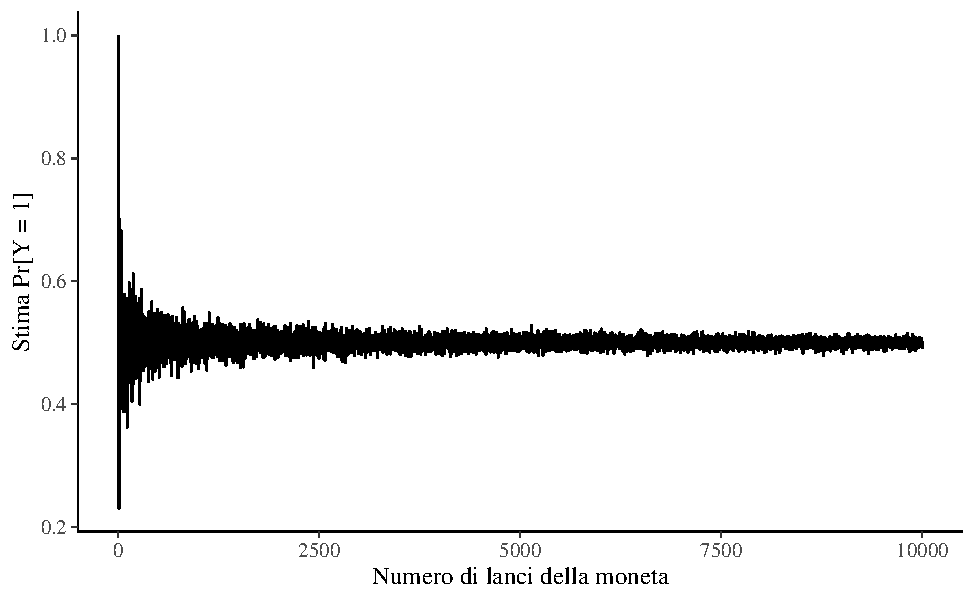
\includegraphics{ds4psy_files/figure-latex/legge-grandi-n-1-1} 

}

\caption{Stima della probabilità di successo in funzione del numero di lanci di una moneta.}\label{fig:legge-grandi-n-1}
\end{figure}

Dato che il grafico \ref{fig:legge-grandi-n-1} espresso su una scala lineare non rivela chiaramente l'andamento della simulazione, imponiamo una scala logaritmica sull'asse delle ascisse (\(x\)). Su scala logaritmica, i valori tra 1 e 10 vengono tracciati all'incirca con la stessa ampiezza che si osserva tra i valori 50 e 700, eccetera.

\begin{Shaded}
\begin{Highlighting}[]
\NormalTok{d }\SpecialCharTok{\%\textgreater{}\%}
  \FunctionTok{ggplot}\NormalTok{(}
    \FunctionTok{aes}\NormalTok{(}\AttributeTok{x =}\NormalTok{ n, }\AttributeTok{y =}\NormalTok{ estimate)}
\NormalTok{  ) }\SpecialCharTok{+}
  \FunctionTok{geom\_line}\NormalTok{() }\SpecialCharTok{+}
  \FunctionTok{scale\_x\_log10}\NormalTok{(}
    \AttributeTok{breaks =} \FunctionTok{c}\NormalTok{(}
      \DecValTok{1}\NormalTok{, }\DecValTok{3}\NormalTok{, }\DecValTok{10}\NormalTok{, }\DecValTok{50}\NormalTok{, }\DecValTok{200}\NormalTok{,}
      \DecValTok{700}\NormalTok{, }\DecValTok{2500}\NormalTok{, }\DecValTok{10000}
\NormalTok{    )}
\NormalTok{  ) }\SpecialCharTok{+}
  \FunctionTok{theme}\NormalTok{(}\AttributeTok{legend.title =} \FunctionTok{element\_blank}\NormalTok{()) }\SpecialCharTok{+}
  \FunctionTok{labs}\NormalTok{(}
    \AttributeTok{x =} \StringTok{"Numero di lanci della moneta"}\NormalTok{,}
    \AttributeTok{y =} \StringTok{"Stima Pr[Y = 1]"}
\NormalTok{  )}
\end{Highlighting}
\end{Shaded}

\begin{figure}

{\centering 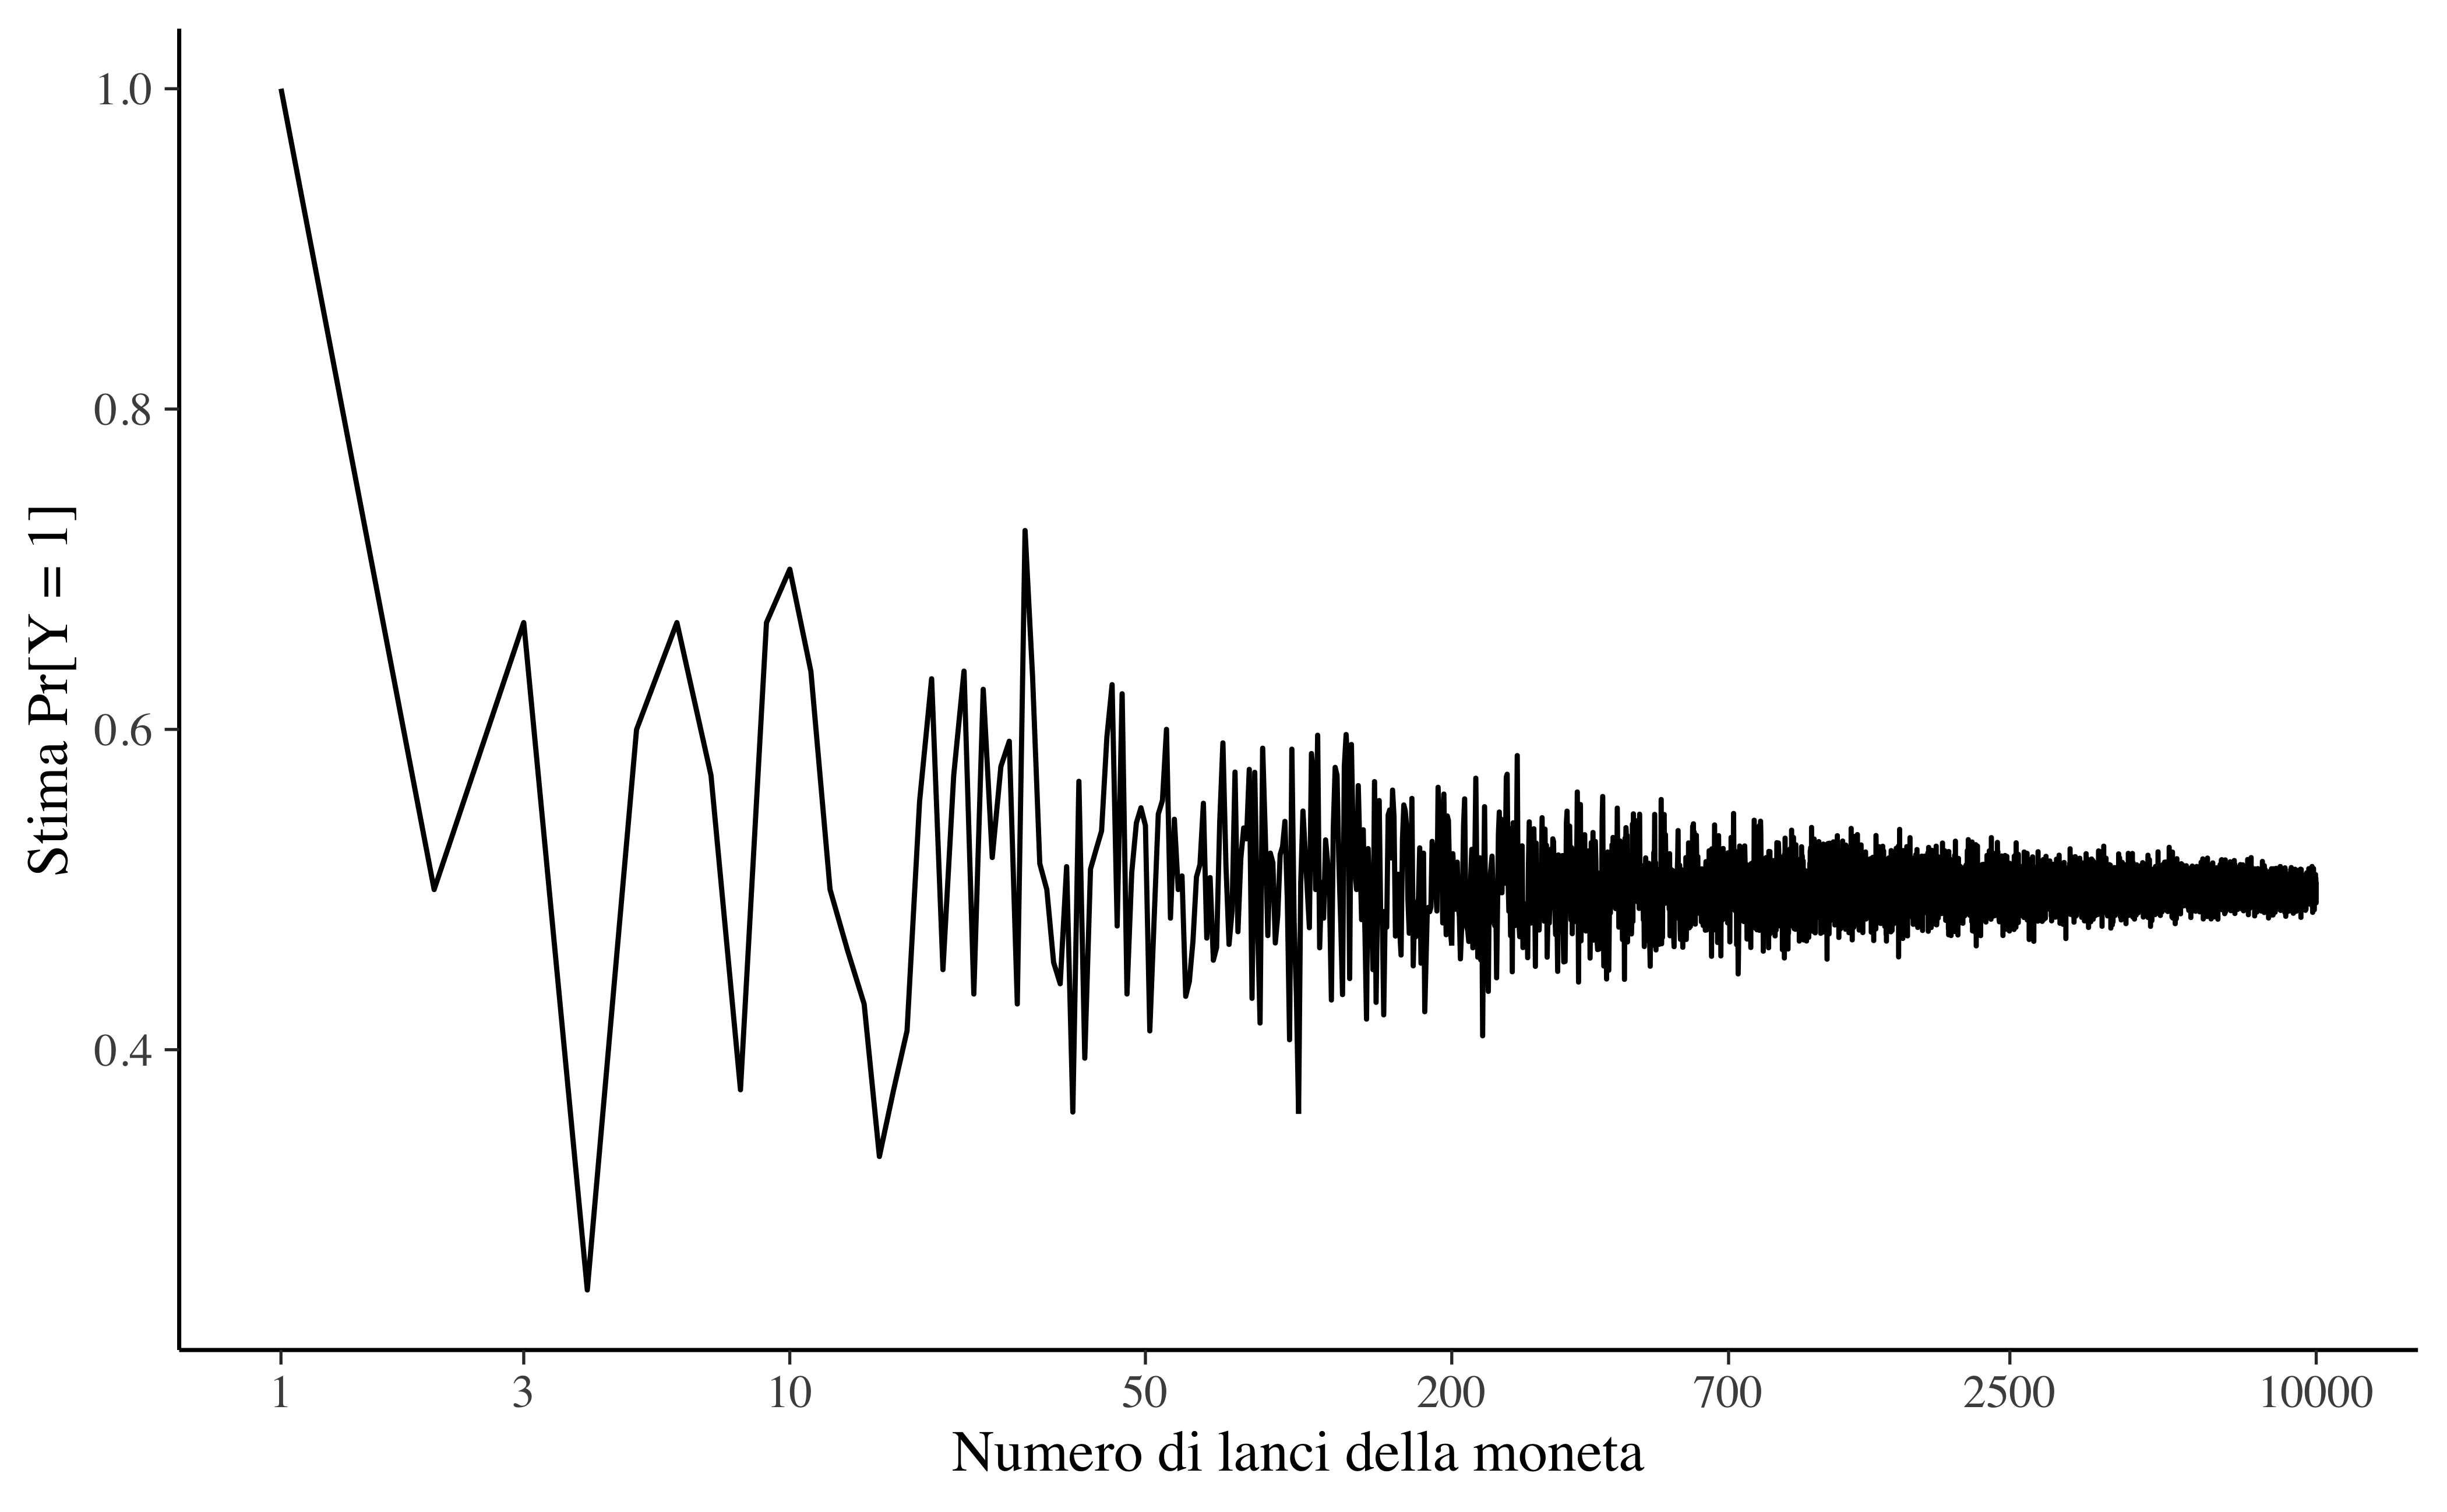
\includegraphics{ds4psy_files/figure-latex/legge-grandi-n-2-1} 

}

\caption{Stima della probabilità di successo in funzione del numero di lanci di una moneta -- scala logaritmica.}\label{fig:legge-grandi-n-2}
\end{figure}

La \emph{legge dei grandi numeri} ci dice che, all'aumentare del numero di ripetizioni dell'esperimento casuale, la media dei risultati ottenuti tende al valore atteso, man mano che vengono eseguite più prove. Nella figura \ref{fig:legge-grandi-n-2} vediamo infatti che, all'aumentare del numero \emph{M} di lanci della moneta, la stima di \(P(Y = 1)\) converge al valore 0.5.

\hypertarget{variabili-casuali-multiple}{%
\section{Variabili casuali multiple}\label{variabili-casuali-multiple}}

Le variabili casuali non esistono isolatamente. Abbiamo iniziato con una singola variabile casuale \emph{Y} che rappresenta il risultato di un singolo, specifico lancio di una moneta equlibrata. Ma supponiamo ora di lanciare la moneta tre volte. I risultati di ciascuno dei tre lanci possono essere rappresentati da una diversa variabile casuale, ad esempio, \(Y_1 , Y_2 , Y_3\). Possiamo assumere che ogni lancio sia indipendente, ovvero che non dipenda dal risultato degli altri lanci. Ognuna di queste variabili \(Y_n\) per \(n \in 1:3\) ha \(P(Y_n =1)=0.5\) e \(P(Y_n =0)=0.5\).

È possibile combinare più variabili casuali usando le operazioni aritmetiche. Se \(Y_1 , Y_2, Y_3\) sono variabili casuali che rappresentano tre lanci di una moneta equilibrata (o un lancio di tre monete equilibrate), possiamo definire la somma di tali variabili casuali come

\[
Z = Y_1 + Y_2 + Y_3.
\]

Possiamo simulare i valori assunti dalla variabile casuale \emph{Z} simulando i valori di \(Y_1, Y_2, Y_3\) per poi sommarli.

\begin{Shaded}
\begin{Highlighting}[]
\NormalTok{y1 }\OtherTok{\textless{}{-}} \FunctionTok{rbinom}\NormalTok{(}\DecValTok{1}\NormalTok{, }\DecValTok{1}\NormalTok{, }\FloatTok{0.5}\NormalTok{)}
\NormalTok{y2 }\OtherTok{\textless{}{-}} \FunctionTok{rbinom}\NormalTok{(}\DecValTok{1}\NormalTok{, }\DecValTok{1}\NormalTok{, }\FloatTok{0.5}\NormalTok{)}
\NormalTok{y3 }\OtherTok{\textless{}{-}} \FunctionTok{rbinom}\NormalTok{(}\DecValTok{1}\NormalTok{, }\DecValTok{1}\NormalTok{, }\FloatTok{0.5}\NormalTok{)}
\FunctionTok{c}\NormalTok{(y1, y2, y3)}
\CommentTok{\#\textgreater{} [1] 1 0 1}
\NormalTok{z }\OtherTok{\textless{}{-}} \FunctionTok{sum}\NormalTok{(}\FunctionTok{c}\NormalTok{(y1, y2, y3))}
\FunctionTok{cat}\NormalTok{(}\StringTok{"z ="}\NormalTok{, z, }\StringTok{"}\SpecialCharTok{\textbackslash{}n}\StringTok{"}\NormalTok{)}
\CommentTok{\#\textgreater{} z = 2}
\end{Highlighting}
\end{Shaded}

ovvero,

\begin{Shaded}
\begin{Highlighting}[]
\NormalTok{y }\OtherTok{\textless{}{-}} \FunctionTok{rep}\NormalTok{(}\ConstantTok{NA}\NormalTok{, }\DecValTok{3}\NormalTok{)}
\ControlFlowTok{for}\NormalTok{ (i }\ControlFlowTok{in} \DecValTok{1}\SpecialCharTok{:}\DecValTok{3}\NormalTok{) \{}
\NormalTok{  y[i] }\OtherTok{\textless{}{-}} \FunctionTok{rbinom}\NormalTok{(}\DecValTok{1}\NormalTok{, }\DecValTok{1}\NormalTok{, }\FloatTok{0.5}\NormalTok{)}
\NormalTok{\}}
\NormalTok{y}
\CommentTok{\#\textgreater{} [1] 0 1 1}
\NormalTok{z }\OtherTok{\textless{}{-}} \FunctionTok{sum}\NormalTok{(y)}
\FunctionTok{cat}\NormalTok{(}\StringTok{"z ="}\NormalTok{, z, }\StringTok{"}\SpecialCharTok{\textbackslash{}n}\StringTok{"}\NormalTok{)}
\CommentTok{\#\textgreater{} z = 2}
\end{Highlighting}
\end{Shaded}

oppure, ancora più semplicemente:

\begin{Shaded}
\begin{Highlighting}[]
\NormalTok{y }\OtherTok{\textless{}{-}} \FunctionTok{rbinom}\NormalTok{(}\DecValTok{3}\NormalTok{, }\DecValTok{1}\NormalTok{, }\FloatTok{0.5}\NormalTok{)}
\NormalTok{y}
\CommentTok{\#\textgreater{} [1] 1 0 1}
\NormalTok{z }\OtherTok{\textless{}{-}} \FunctionTok{sum}\NormalTok{(y)}
\FunctionTok{cat}\NormalTok{(}\StringTok{"z ="}\NormalTok{, z, }\StringTok{"}\SpecialCharTok{\textbackslash{}n}\StringTok{"}\NormalTok{)}
\CommentTok{\#\textgreater{} z = 2}
\end{Highlighting}
\end{Shaded}

Possiamo ripetere questa simulazione \(M = 1e5\) volte:

\begin{Shaded}
\begin{Highlighting}[]
\NormalTok{M }\OtherTok{\textless{}{-}} \FloatTok{1e5}
\NormalTok{z }\OtherTok{\textless{}{-}} \FunctionTok{rep}\NormalTok{(}\ConstantTok{NA}\NormalTok{, M)}
\ControlFlowTok{for}\NormalTok{ (i }\ControlFlowTok{in} \DecValTok{1}\SpecialCharTok{:}\NormalTok{M) \{}
\NormalTok{  y }\OtherTok{\textless{}{-}} \FunctionTok{rbinom}\NormalTok{(}\DecValTok{3}\NormalTok{, }\DecValTok{1}\NormalTok{, }\FloatTok{0.5}\NormalTok{)}
\NormalTok{  z[i] }\OtherTok{\textless{}{-}} \FunctionTok{sum}\NormalTok{(y)}
\NormalTok{\}}
\end{Highlighting}
\end{Shaded}

e calcolare una stima della probabilità che la variabile casuale \(Z\) assuma i valori 0, 1, 2, 3:

\begin{Shaded}
\begin{Highlighting}[]
\FunctionTok{table}\NormalTok{(z) }\SpecialCharTok{/}\NormalTok{ M}
\CommentTok{\#\textgreater{} z}
\CommentTok{\#\textgreater{}      0      1      2      3 }
\CommentTok{\#\textgreater{} 0.1258 0.3750 0.3748 0.1244}
\end{Highlighting}
\end{Shaded}

Nel caso di 4 monete equilibrate, avremo:

\begin{Shaded}
\begin{Highlighting}[]
\NormalTok{M }\OtherTok{\textless{}{-}} \FloatTok{1e5}
\NormalTok{z }\OtherTok{\textless{}{-}} \FunctionTok{rep}\NormalTok{(}\ConstantTok{NA}\NormalTok{, M)}
\ControlFlowTok{for}\NormalTok{ (i }\ControlFlowTok{in} \DecValTok{1}\SpecialCharTok{:}\NormalTok{M) \{}
\NormalTok{  y }\OtherTok{\textless{}{-}} \FunctionTok{rbinom}\NormalTok{(}\DecValTok{4}\NormalTok{, }\DecValTok{1}\NormalTok{, }\FloatTok{0.5}\NormalTok{)}
\NormalTok{  z[i] }\OtherTok{\textless{}{-}} \FunctionTok{sum}\NormalTok{(y)}
\NormalTok{\}}
\FunctionTok{table}\NormalTok{(z) }\SpecialCharTok{/}\NormalTok{ M}
\CommentTok{\#\textgreater{} z}
\CommentTok{\#\textgreater{}       0       1       2       3       4 }
\CommentTok{\#\textgreater{} 0.06340 0.24917 0.37360 0.25022 0.06361}
\end{Highlighting}
\end{Shaded}

Una variabile casuale le cui modalità possono essere costituite solo da numeri interi è detta \emph{variabile casuale discreta}:

\[
\mathbb{Z} = \dots, -2, -1, 0, 1, 2, \dots
\]

\hypertarget{sec:fun-mass-prob}{%
\section{Funzione di massa di probabilità}\label{sec:fun-mass-prob}}

È conveniente avere una funzione che associa ogni possibile valore di una variabile casuale alla sua probabilità. In generale, ciò è possibile se e solo se la variabile casuale è discreta, così com'è stata definita nel Paragrafo precedente.

Ad esempio, se consideriamo \(Z = Y_1 + \dots + Y_4\) come il numero di risultati ``testa'' in 4 lanci della moneta, allora possiamo definire la seguente funzione:

\[
\begin{array}{rclll}
p_Z(0) & = & 1/16 & & \mathrm{TTTT}
\\
p_Z(1) & = & 4/16 & & \mathrm{HTTT, THTT, TTHT, TTTH}
\\
p_Z(2) & = & 6/16 & & \mathrm{HHTT, HTHT, HTTH, THHT, THTH, TTTH}
\\
p_Z(3) & = & 4/16 & & \mathrm{HHHT, HHTH, HTHH, THHH}
\\
p_Z(4) & = & 1/16 & & \mathrm{HHHH}
\end{array}
\]

Il lancio di quattro monete può produrre sedici possibili risultati. Dato che i lanci sono indipendenti e le monete sono equilibrate, ogni possibile risultato è ugualmente probabile. Nella tabella in alto, le sequenze dei risultati possibili del lancio delle 4 monete sono riportate nella colonna più a destra. Le probabilità si ottengono dividendo il numero di sequenze che producono lo stesso numero di eventi testa per il numero dei risultati possibili.

La funzione \(p_Z\) è stata costruita per mappare un valore \(u\) per \(Z\) alla probabilità dell'evento \(Z = u\). Convenzionalmente, queste probabilità sono scritte come

\[
P_Z(z) = \mbox{P}(Z = z).
\]

La parte a destra dell'uguale si può leggere come: ``la probabilità che la variabile casuale \(Z\) assuma il valore \(z\)''.

Una funzione definita come sopra è detta \emph{funzione di massa di probabilità} della variabile casuale \(Z\). Ad ogni variabile casuale discreta è associata un'unica funzione di massa di probabilità.

Una rappresentazione grafica della stima della funzione di massa di probabilità per l'esperimento casuale del lancio di quattro monete equilibrate è fornita nella figura \ref{fig:barplot-mdf-4coins}.

\begin{Shaded}
\begin{Highlighting}[]
\FunctionTok{set.seed}\NormalTok{(}\DecValTok{1234}\NormalTok{)}
\NormalTok{M }\OtherTok{\textless{}{-}} \FloatTok{1e5}
\NormalTok{nflips }\OtherTok{\textless{}{-}} \DecValTok{4}
\NormalTok{u }\OtherTok{\textless{}{-}} \FunctionTok{rbinom}\NormalTok{(M, nflips, }\FloatTok{0.5}\NormalTok{)}
\NormalTok{x }\OtherTok{\textless{}{-}} \DecValTok{0}\SpecialCharTok{:}\NormalTok{nflips}
\NormalTok{y }\OtherTok{\textless{}{-}} \FunctionTok{rep}\NormalTok{(}\ConstantTok{NA}\NormalTok{, nflips }\SpecialCharTok{+} \DecValTok{1}\NormalTok{)}
\ControlFlowTok{for}\NormalTok{ (n }\ControlFlowTok{in} \DecValTok{0}\SpecialCharTok{:}\NormalTok{nflips) \{}
\NormalTok{  y[n }\SpecialCharTok{+} \DecValTok{1}\NormalTok{] }\OtherTok{\textless{}{-}} \FunctionTok{sum}\NormalTok{(u }\SpecialCharTok{==}\NormalTok{ n) }\SpecialCharTok{/}\NormalTok{ M}
\NormalTok{\}}
\NormalTok{bar\_plot }\OtherTok{\textless{}{-}}
  \FunctionTok{data.frame}\NormalTok{(}\AttributeTok{Z =}\NormalTok{ x, }\AttributeTok{count =}\NormalTok{ y) }\SpecialCharTok{\%\textgreater{}\%}
  \FunctionTok{ggplot}\NormalTok{(}
    \FunctionTok{aes}\NormalTok{(}\AttributeTok{x =}\NormalTok{ Z, }\AttributeTok{y =}\NormalTok{ count)}
\NormalTok{  ) }\SpecialCharTok{+}
  \FunctionTok{geom\_bar}\NormalTok{(}\AttributeTok{stat =} \StringTok{"identity"}\NormalTok{) }\SpecialCharTok{+}
  \FunctionTok{scale\_x\_continuous}\NormalTok{(}
    \AttributeTok{breaks =} \DecValTok{0}\SpecialCharTok{:}\DecValTok{4}\NormalTok{,}
    \AttributeTok{labels =} \FunctionTok{c}\NormalTok{(}\DecValTok{0}\NormalTok{, }\DecValTok{1}\NormalTok{, }\DecValTok{2}\NormalTok{, }\DecValTok{3}\NormalTok{, }\DecValTok{4}\NormalTok{)}
\NormalTok{  ) }\SpecialCharTok{+}
  \FunctionTok{labs}\NormalTok{(}
    \AttributeTok{y =} \StringTok{"Probabilità stimata Pr[Z = z]"}
\NormalTok{  )}
\NormalTok{bar\_plot}
\end{Highlighting}
\end{Shaded}

\begin{figure}

{\centering 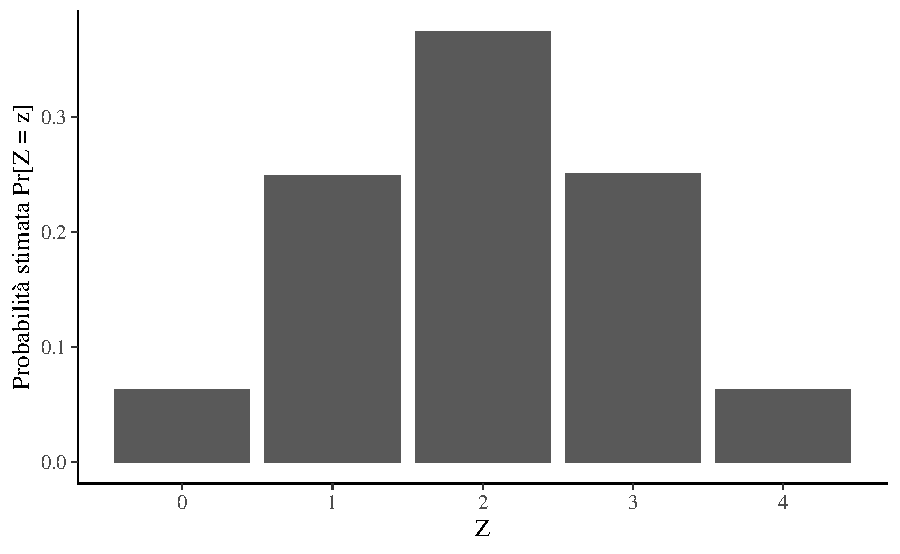
\includegraphics{ds4psy_files/figure-latex/barplot-mdf-4coins-1} 

}

\caption{Grafico di $M = 100\,000$ simulazioni della funzione di massa di probabilità di una variabile casuale definita come il numero di teste in quattro lanci di una moneta equilibrata.}\label{fig:barplot-mdf-4coins}
\end{figure}

Se \(A\) è un sottoinsieme della variabile casuale \(Z\), allora denotiamo con \(P_{z}(A)\) la probabilità assegnata ad \(A\) dalla distribuzione \(P_{z}\). Mediante una distribuzione di probabilità \(P_{z}\) è dunque possibile determinare la probabilità di ciascun sottoinsieme \(A \subset Z\) come

\[
P_{z}(A) = \sum_{z \in A} P_{z}(Z).
\]

\begin{example}
Nel caso dell'esempio discusso nella Sezione \ref{sec:fun-mass-prob}, la probabilità che la variabile casuale \(Z\) sia un numero dispari è

\[
P(\text{Z è un numero dispari}) = P_{z}(Z = 1) + P_{z}(Z = 3) = \frac{4}{16} + \frac{4}{16} = \frac{1}{2}.
\]
\end{example}

\hypertarget{commenti-e-considerazioni-finali}{%
\section*{Commenti e considerazioni finali}\label{commenti-e-considerazioni-finali}}


In questo capitolo abbiamo visto come si costruisce lo spazio campione di un esperimento casuale, quali sono le proprietà di base della probabilità e come si assegnano le probabilità agli eventi definiti sopra uno spazio campione discreto. Abbiamo anche introdotto le nozioni di ``variabile casuale'', ovvero di una variabile che prende i suoi valori casualmente. E abbiamo descritto il modo di specificare la probabilità con cui sono presi i differenti valori, ovvero la funzione di distribuzione probabilistica \(F(X) = P(X < x)\), e la funzione di massa di probabilità. Le procedure di analisi dei dati psicologici che discuteremo in seguito faranno un grande uso di questi concetti e della notazione qui introdotta.

\hypertarget{chapter-sintesi-distr-post}{%
\chapter{Sintesi a posteriori}\label{chapter-sintesi-distr-post}}

La distribuzione a posteriori è un modo per descrivere il nostro grado di incertezza rispetto al parametro incognito (o rispetto ai parametri incogniti) oggetto dell'inferenza. La distribuzione a posteriori contiene tutte le informazioni disponibili sui possibili valori del parametro. Se il parametro esaminato è monodimensionale (o bidimensionale) è possibile fornire un grafico di tutta la distribuzione a posteriori \(p(\theta \mid y)\). Tuttavia, spesso vogliamo anche giungere ad una sintesi numerica della distribuzione a posteriori, soprattutto se il vettore dei parametri ha più di due dimensioni. A a questo proposito è possibile utilizzare le consuete statistiche descrittive, come media, mediana, moda, varianza, deviazione standard e i quantili. In alcuni casi, queste statistiche descrittive sono più facili da presentare e interpretare rispetto alla rappresentazione grafica della distribuzione a posteriori.

La stima puntuale della tendenza centrale della distribuzione a posteriori fornisce informazioni su quello che può essere considerato come il ``valore più plausibile'' del parametro. L'intervallo di credibilità fornisce invece un'indicazione dell'ampiezza dell'intervallo che contiene una determinata quota della massa della distribuzione a posteriori del parametro.

\hypertarget{stima-puntuale}{%
\section{Stima puntuale}\label{stima-puntuale}}

Per sintetizzare la distribuzione a posteriori in modo da giungere ad una stima puntuale di \(\theta\) si è soliti scegliere tra moda, mediana o media a seconda del tipo di distribuzione con cui si ha a che fare e della sua forma. Ogni stima puntuale ha una sua interpretazione.

\begin{itemize}
\tightlist
\item
  La media è il valore atteso a posteriori del parametro.
\item
  La moda può essere interpretata come il singolo valore più credibile (``più plausibile'') del parametro, alla luce dei dati, ovvero il valore per il parametro \(\theta\) che massimizza la distribuzione a posteriori. Per questa ragione la moda viene detta \emph{massimo a posteriori}, MAP. Il limite della moda quale statistica riassuntiva della distribuzione a posteriori è che, talvolta, tale distribuzione è multimodale e il MAP non è necessariamente il valore ``più credibile''.
\item
  La mediana è il valore del parametro tale per cui, su entrambi i lati di essa, giace il 50\% della massa di probabilità a posteriori.
\end{itemize}

La misura di variabilità del parametro è la \emph{varianza a posteriori} la quale, nel caso di una distribuzione a posteriori ottenuta per via numerica, si calcola con la formula della varianza che conosciamo rispetto alla tendenza centrale data dalla media a posteriori. La radice quadrata della varianza a posteriori è la \emph{deviazione standard a posteriori} che descrive l'incertezza a posteriori circa il parametro di interesse nella stessa unità di misura dei dati.

Le procedure bayesiane basate sui metodi MCMC utilizzano un numero finito di campioni dalla distribuzione stazionaria, e una tale caratteristica della simulazione introduce un ulteriore livello di incertezza nella stima del parametro. L'\emph{errore standard della stima} (in inglese \emph{Monte Carlo standard error}, MCSE) misura l'accuratezza della simulazione. La deviazione standard a posteriori e l'errore standard della stima sono due concetti completamente diversi. La deviazione standard a posteriori descrive l'incertezza circa il parametro (l'ampiezza della distribuzione a posteriori) ed è una funzione della dimensione del campione; il MCSE descrive invece l'incertezza nella stima del parametro dovuta alla simulazione MCMC ed è una funzione del numero di iterazioni nella simulazione.

\hypertarget{intervallo-di-credibilituxe0}{%
\section{Intervallo di credibilità}\label{intervallo-di-credibilituxe0}}

Molto spesso la stima puntuale è accompagnata da una stima intervallare (abbiamo già incontrato questo aspetto nel Capitolo \ref{ch-distr-coniugate} discutendo lo schema beta-binomiale). Nella statistica bayesiana, se il parametro \(\theta \in \Theta\) è monodimensionale, si dice \emph{intervallo di credibilità} un intervallo di valori \(I_{\alpha}\) che contiene la proporzione \(1 - \alpha\) della massa di probabilità della funzione a posteriori:

\begin{equation}
p(\Theta \in I_{\alpha} \mid y) = 1 - \alpha.
\label{eq:credibint}
\end{equation}

L'intervallo di credibilità ha lo scopo di esprimere il nostro grado di incertezza riguardo la stima del parametro. Se il parametro \(\theta\) è multidimensionale, si parla invece di ``regione di credibilità''.

La condizione \eqref{eq:credibint} non determina un unico intervallo di credibilità al \((1 - \alpha) \cdot 100\%\). In realtà esiste un numero infinito di tali intervalli. Ciò significa che dobbiamo definire alcune condizioni aggiuntive per la scelta dell'intervallo di credibilità. Esaminiamo due delle condizioni aggiuntive più comuni.

\hypertarget{intervallo-di-credibilituxe0-a-code-uguali}{%
\subsection{Intervallo di credibilità a code uguali}\label{intervallo-di-credibilituxe0-a-code-uguali}}

Un intervallo di credibilità \emph{a code uguali} a livello \(\alpha\) è un intervallo

\[
I_{\alpha} = [q_{\alpha/2}, 1 - q_{\alpha/2}],
\]

dove \(q_z\) è un quantile \(z\) della distribuzione a posteriori. Per esempio, l'intervallo di credibilità a code uguali al 95\% è un intervallo

\[
I_{0.05} = [q_{0.025}, q_{0.975}]
\]

che lascia il 2.5\% della massa di densità a posteriori in ciascuna coda.

\hypertarget{intervallo-di-credibilituxe0-a-densituxe0-a-posteriori-piuxf9-alta}{%
\subsection{Intervallo di credibilità a densità a posteriori più alta}\label{intervallo-di-credibilituxe0-a-densituxe0-a-posteriori-piuxf9-alta}}

Nell'intervallo di credibilità a code uguali alcuni valori del parametro che sono inclusi nell'intervallo possono avere una credibilità a posteriori più bassa rispetto a quelli esterni all'intervallo. L'intrevallo di credibilità \emph{a densità a posteriori più alta} (in inglese \emph{High Posterior Density Interval}, HPD) è invece costruito in modo tale da assicurare di includere nell'intervallo tutti i valori \(\theta\) che sono a posteriori maggiormente credibili. Graficamente questo intervallo può essere ricavato tracciando una linea orizzontale sulla rappresentazione della distribuzione a posteriori e regolando l'altezza della linea in modo tale che l'area sottesa alla curva sia pari a \(1 - \alpha\). Questo tipo di intervallo è il più stretto possibile, tra tutti i possibili intervalli di credibilità allo stesso livello di fiducia. Se la distribuzione a posteriori è simmetrica unimodale, l'intervallo di credibilità a densità a posteriori più alta corrisponde all'intervallo di credibilità a code uguali.

\hypertarget{interpretazione}{%
\subsection{Interpretazione}\label{interpretazione}}

L'interpretazione dell'intervallo di credibilità è molto intuitiva: l'intervallo di credibilità è un intervallo di valori all'interno del quale cade il valore del parametro incognito con un particolare livello di probabilità soggettiva. Possiamo dire che, dopo aver visto i dati crediamo, con un determinato livello di probabilità soggettiva, che il valore del parametro (ad esempio, la dimensione dell'effetto di un trattamento) abbia un valore compreso all'interno dell'intervallo che è stato calcolato, laddove per probabilità soggettiva intendiamo ``il grado di fiducia che lo sperimentatore ripone nel verificarsi di un evento''. Gli intervalli di credibilità si calcolano con un software.

\hypertarget{un-esempio-concreto}{%
\section{Un esempio concreto}\label{un-esempio-concreto}}

Per fare un esempio pratico, consideriamo nuovamente i valori del BDI-II dei 30 soggetti clinici di \citet{zetschefuture2019}:

\begin{Shaded}
\begin{Highlighting}[]
\FunctionTok{suppressPackageStartupMessages}\NormalTok{(}\FunctionTok{library}\NormalTok{(}\StringTok{"bayesrules"}\NormalTok{))}

\NormalTok{df }\OtherTok{\textless{}{-}} \FunctionTok{tibble}\NormalTok{(}
  \AttributeTok{y =} \FunctionTok{c}\NormalTok{(}
    \DecValTok{26}\NormalTok{, }\DecValTok{35}\NormalTok{, }\DecValTok{30}\NormalTok{, }\DecValTok{25}\NormalTok{, }\DecValTok{44}\NormalTok{, }\DecValTok{30}\NormalTok{, }\DecValTok{33}\NormalTok{, }\DecValTok{43}\NormalTok{, }\DecValTok{22}\NormalTok{, }\DecValTok{43}\NormalTok{,}
    \DecValTok{24}\NormalTok{, }\DecValTok{19}\NormalTok{, }\DecValTok{39}\NormalTok{, }\DecValTok{31}\NormalTok{, }\DecValTok{25}\NormalTok{, }\DecValTok{28}\NormalTok{, }\DecValTok{35}\NormalTok{, }\DecValTok{30}\NormalTok{, }\DecValTok{26}\NormalTok{, }\DecValTok{31}\NormalTok{,}
    \DecValTok{41}\NormalTok{, }\DecValTok{36}\NormalTok{, }\DecValTok{26}\NormalTok{, }\DecValTok{35}\NormalTok{, }\DecValTok{33}\NormalTok{, }\DecValTok{28}\NormalTok{, }\DecValTok{27}\NormalTok{, }\DecValTok{34}\NormalTok{, }\DecValTok{27}\NormalTok{, }\DecValTok{22}
\NormalTok{  )}
\NormalTok{)}
\end{Highlighting}
\end{Shaded}

Un valore BDI-II \(\geq 30\) indica la presenza di un livello ``grave'' di depressione. Nel campione clinico di \citet{zetschefuture2019},

\begin{Shaded}
\begin{Highlighting}[]
\FunctionTok{sum}\NormalTok{(df}\SpecialCharTok{$}\NormalTok{y }\SpecialCharTok{\textgreater{}} \DecValTok{29}\NormalTok{)}
\CommentTok{\#\textgreater{} [1] 17}
\end{Highlighting}
\end{Shaded}

17 pazienti su 30 manifestano un livello grave di depressione.

Supponiamo di volere stimare la distribuzione a posteriori della probabilità \(\theta\) di depressione ``grave'' nei pazienti clinici, così come viene misurata dal test BDI-II, imponendo su \(\theta\) una distribuzione a priori \(\mbox{Beta}(8, 2)\).

Sappiamo che il modello Beta-Binomiale può essere espresso nella forma seguente:

\begin{align}
Y | \theta & \sim \mbox{Bin}(30, \theta) \notag\\
\theta & \sim \mbox{Beta}(8, 2) \notag
\end{align}

con una corrispondente distribuzione a posteriori \(\mbox{Beta}(25, 15)\):

\begin{equation}
f(\theta | y = 17) = \frac{\Gamma(25 + 15)}{\Gamma(25)\Gamma(15)}\theta^{25-1} (1-\theta)^{15-1} \;\; \text{ for } \theta \in [0,1] \; .
\label{eq:post-beta-25-15}
\end{equation}

\begin{Shaded}
\begin{Highlighting}[]
\FunctionTok{plot\_beta\_binomial}\NormalTok{(}\AttributeTok{alpha =} \DecValTok{8}\NormalTok{, }\AttributeTok{beta =} \DecValTok{2}\NormalTok{, }\AttributeTok{y =} \DecValTok{17}\NormalTok{, }\AttributeTok{n =} \DecValTok{30}\NormalTok{)}
\end{Highlighting}
\end{Shaded}

\begin{center}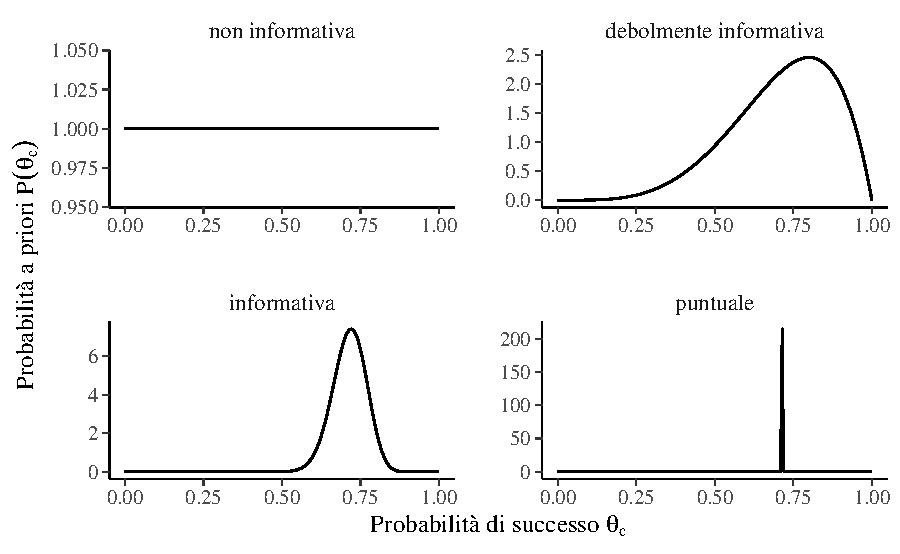
\includegraphics{ds4psy_files/figure-latex/unnamed-chunk-19-1} \end{center}

\hypertarget{stime-puntuali-della-distribuzione-a-posteriori}{%
\subsection{Stime puntuali della distribuzione a posteriori}\label{stime-puntuali-della-distribuzione-a-posteriori}}

Una volta trovata l'intera distribuzione a posteriori, quale valore di sintesi è necessario riportare? Questa sembra una domanda innocente, ma in realtà è una domanda a cui è difficile rispondere. La stima bayesiana dei parametri è fornita dall'intera distribuzione a posteriori, che non è un singolo numero, ma una funzione che mappa ciascun valore del parametro ad un valore di plausibilità. Quindi non è necessario scegliere una stima puntuale. In linea di principio, una stima puntuale non è quasi mai necessaria ed è spesso dannosa in quanto comporta una perdita di informazioni.

Tuttavia talvolta una tale sintesi è richiesta. Diverse risposte sono allora possibili. La media della distribuzione a posteriori per \(\theta\) è

\[
\E(\pi \mid y = 17) = \frac{\alpha}{\alpha + \beta} = \frac{25}{25+15} = 0.625.
\]

Una stima del massimo della probabilità a posteriori, o brevemente massimo a posteriori, MAP (da \emph{maximum a posteriori probability}), è la moda della distribuzione a posteriori. Nel caso presente, una stima del MAP può essere ottenuta nel modo seguente:

\[
\Mo(\pi \mid y = 17) = \frac{\alpha-1}{\alpha + \beta-2} = \frac{25-1}{25+15-2} = 0.6316.
\]

Gli stessi risultati si ottiengono usando la chiamata a \texttt{bayesrules::summarize\_beta\_binomial()}:

\begin{Shaded}
\begin{Highlighting}[]
\FunctionTok{summarize\_beta\_binomial}\NormalTok{(}\AttributeTok{alpha =} \DecValTok{8}\NormalTok{, }\AttributeTok{beta =} \DecValTok{2}\NormalTok{, }\AttributeTok{y =} \DecValTok{17}\NormalTok{, }\AttributeTok{n =} \DecValTok{30}\NormalTok{)}
\CommentTok{\#\textgreater{}       model alpha beta  mean   mode      var      sd}
\CommentTok{\#\textgreater{} 1     prior     8    2 0.800 0.8750 0.014545 0.12060}
\CommentTok{\#\textgreater{} 2 posterior    25   15 0.625 0.6316 0.005716 0.07561}
\end{Highlighting}
\end{Shaded}

La mediana si ottiene con

\begin{Shaded}
\begin{Highlighting}[]
\FunctionTok{qbeta}\NormalTok{(.}\DecValTok{5}\NormalTok{, }\AttributeTok{shape1 =} \DecValTok{25}\NormalTok{, }\AttributeTok{shape2 =} \DecValTok{15}\NormalTok{)}
\CommentTok{\#\textgreater{} [1] 0.6271}
\end{Highlighting}
\end{Shaded}

\hypertarget{intervallo-di-credibilituxe0-1}{%
\subsection{Intervallo di credibilità}\label{intervallo-di-credibilituxe0-1}}

È più comune sintetizzare la distribuzione a posteriori mediante l'intervallo di credibilità. Per esempio, l'intervallo di credibilità a code uguali al 95\%

\begin{Shaded}
\begin{Highlighting}[]
\FunctionTok{plot\_beta\_ci}\NormalTok{(}\AttributeTok{alpha =} \DecValTok{25}\NormalTok{, }\AttributeTok{beta =} \DecValTok{15}\NormalTok{, }\AttributeTok{ci\_level =} \FloatTok{0.95}\NormalTok{)}
\end{Highlighting}
\end{Shaded}

\begin{center}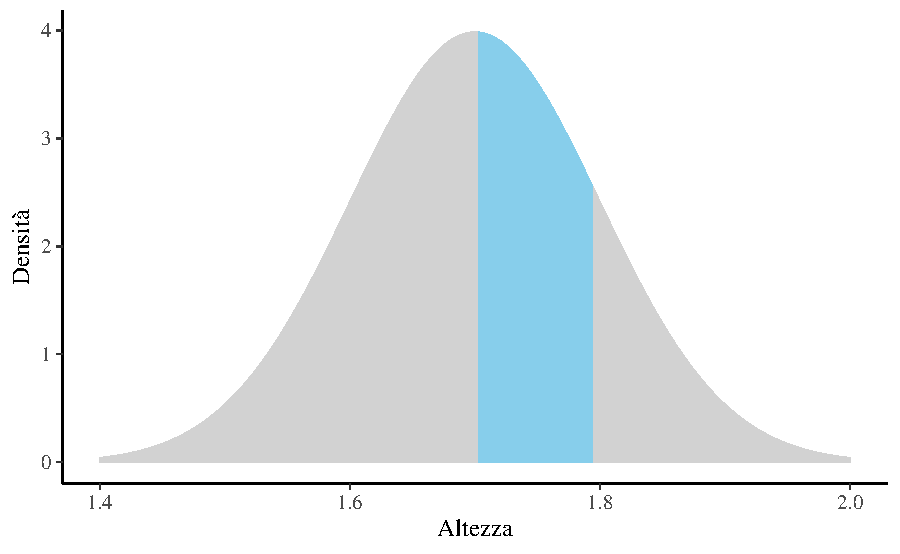
\includegraphics{ds4psy_files/figure-latex/unnamed-chunk-22-1} \end{center}

è dato dalla chiamata

\begin{Shaded}
\begin{Highlighting}[]
\FunctionTok{qbeta}\NormalTok{(}\FunctionTok{c}\NormalTok{(}\FloatTok{0.025}\NormalTok{, }\FloatTok{0.975}\NormalTok{), }\DecValTok{25}\NormalTok{, }\DecValTok{15}\NormalTok{)}
\CommentTok{\#\textgreater{} [1] 0.4718 0.7664}
\end{Highlighting}
\end{Shaded}

Il calcolo precedente evidenzia l'interpretazione intuitiva dell'intervallo di credibilità. Tale intervallo, infatti, può essere interpretato come la probabilità che \(\theta\) assuma valori compresi tra 0.472 e 0.766:

\[
P(\theta \in (0.472, 0.766) | Y = 17) = \int_{0.472}^{0.766} f(\theta \mid y=17) d\theta = 0.95,
\]

ovvero

\begin{Shaded}
\begin{Highlighting}[]
\NormalTok{postFun }\OtherTok{\textless{}{-}} \ControlFlowTok{function}\NormalTok{(theta) \{}
  \FunctionTok{gamma}\NormalTok{(}\DecValTok{25} \SpecialCharTok{+} \DecValTok{15}\NormalTok{) }\SpecialCharTok{/}
\NormalTok{    (}\FunctionTok{gamma}\NormalTok{(}\DecValTok{25}\NormalTok{) }\SpecialCharTok{*} \FunctionTok{gamma}\NormalTok{(}\DecValTok{15}\NormalTok{)) }\SpecialCharTok{*}\NormalTok{ theta}\SpecialCharTok{\^{}}\DecValTok{24} \SpecialCharTok{*}\NormalTok{ (}\DecValTok{1} \SpecialCharTok{{-}}\NormalTok{ theta)}\SpecialCharTok{\^{}}\DecValTok{14}
\NormalTok{\}}
\FunctionTok{integrate}\NormalTok{(}
\NormalTok{  postFun,}
  \AttributeTok{lower =} \FloatTok{0.4717951}\NormalTok{,}
  \AttributeTok{upper =} \FloatTok{0.7663607}
\NormalTok{)}\SpecialCharTok{$}\NormalTok{value}
\CommentTok{\#\textgreater{} [1] 0.95}
\end{Highlighting}
\end{Shaded}

Possiamo costruire diversi intervalli di credibilità a code equivalenti. Ad esempio, l'intervallo di credibilità compreso tra il 25-esimo e il 75-esimo percentile è

\begin{Shaded}
\begin{Highlighting}[]
\FunctionTok{qbeta}\NormalTok{(}\FunctionTok{c}\NormalTok{(}\FloatTok{0.25}\NormalTok{, }\FloatTok{0.75}\NormalTok{), }\DecValTok{25}\NormalTok{, }\DecValTok{15}\NormalTok{)}
\CommentTok{\#\textgreater{} [1] 0.5744 0.6779}
\end{Highlighting}
\end{Shaded}

ovvero, abbiamo una certezza a posteriori del 50\% che la probabilità di depressione grave tra i pazienti clinici sia un valore compreso tra 0.57 e 0.68.

Non esiste un livello credibile ``corretto''. I ricercatori, utilizzano vari livelli, ad esempio 50\%, 80\% o 95\%, a seconda del contesto dell'analisi. Ciascuno di questi intervalli fornisce un'immagine diversa della nostra comprensione della distribuzione a posteriori del parametro di interesse.

Non è inoltre necessario riportare l'intervallo di credibilità a code uguali. Se la distribuzione a posteriori è fortemente asimmetrica è più sensato riportare l'intervallo di credibilità a densità a posteriori più alta. L'intervallo HPD risulta più semplice da determinare quando la distribuzione a posteriori viene approssimata con il metodo MCMC.

\hypertarget{probabilituxe0-della-distribuzione-a-posteriori}{%
\subsection{Probabilità della distribuzione a posteriori}\label{probabilituxe0-della-distribuzione-a-posteriori}}

Il test di ipotesi è un compito comune dell'analisi della distribuzione a posteriori (si veda anche il Capitolo \ref{ch-distr-coniugate}). Supponiamo che si voglia conoscere la probabilità a posteriori che \(\theta\) sia superiore a 0.5. Per sapere quanto credibile sia l'evento \(\theta > 0.5\) possiamo calcolare il seguente integrale:

\[
P(\theta > 0.5 \; \mid \; y = 17) = \int_{0.5}^{1}f(\theta \mid y=17)d\theta \;,
\]

dove \(f(\cdot)\) è la distribuzione \(\mbox{\Beta}(25, 15)\):

\begin{Shaded}
\begin{Highlighting}[]
\FunctionTok{pbeta}\NormalTok{(}\FloatTok{0.5}\NormalTok{, }\AttributeTok{shape1 =} \DecValTok{25}\NormalTok{, }\AttributeTok{shape2 =} \DecValTok{15}\NormalTok{, }\AttributeTok{lower.tail =} \ConstantTok{FALSE}\NormalTok{)}
\CommentTok{\#\textgreater{} [1] 0.9459}
\end{Highlighting}
\end{Shaded}

il che è equivalente a:

\begin{Shaded}
\begin{Highlighting}[]
\NormalTok{postFun }\OtherTok{\textless{}{-}} \ControlFlowTok{function}\NormalTok{(theta) \{}
  \FunctionTok{gamma}\NormalTok{(}\DecValTok{25} \SpecialCharTok{+} \DecValTok{15}\NormalTok{) }\SpecialCharTok{/}\NormalTok{ (}\FunctionTok{gamma}\NormalTok{(}\DecValTok{25}\NormalTok{) }\SpecialCharTok{*} \FunctionTok{gamma}\NormalTok{(}\DecValTok{15}\NormalTok{)) }\SpecialCharTok{*}\NormalTok{ theta}\SpecialCharTok{\^{}}\DecValTok{24} \SpecialCharTok{*}\NormalTok{ (}\DecValTok{1} \SpecialCharTok{{-}}\NormalTok{ theta)}\SpecialCharTok{\^{}}\DecValTok{14}
\NormalTok{\}}
\FunctionTok{integrate}\NormalTok{(}
\NormalTok{  postFun,}
  \AttributeTok{lower =} \FloatTok{0.5}\NormalTok{,}
  \AttributeTok{upper =} \DecValTok{1}
\NormalTok{)}\SpecialCharTok{$}\NormalTok{value}
\CommentTok{\#\textgreater{} [1] 0.9459}
\end{Highlighting}
\end{Shaded}

È anche possibile formulare un test di ipotesi contrastando due ipotesi contrapposte. Per esempio, \(H_1: \theta \geq 0.5\) e \(H_2: \theta < 0.5\). Ciò consente di calcolare l'\emph{odds a posteriori} di \(\theta > 0.5\):

\begin{equation}
\text{poterior odds} = \frac{H_1 \mid y = 17}{H_2 \mid y = 17}
\end{equation}

ovvero

\begin{Shaded}
\begin{Highlighting}[]
\NormalTok{posterior\_odds }\OtherTok{\textless{}{-}}
  \FunctionTok{pbeta}\NormalTok{(}\FloatTok{0.5}\NormalTok{, }\AttributeTok{shape1 =} \DecValTok{25}\NormalTok{, }\AttributeTok{shape2 =} \DecValTok{15}\NormalTok{, }\AttributeTok{lower.tail =} \ConstantTok{FALSE}\NormalTok{) }\SpecialCharTok{/}
    \FunctionTok{pbeta}\NormalTok{(}\FloatTok{0.5}\NormalTok{, }\AttributeTok{shape1 =} \DecValTok{25}\NormalTok{, }\AttributeTok{shape2 =} \DecValTok{15}\NormalTok{, }\AttributeTok{lower.tail =} \ConstantTok{TRUE}\NormalTok{)}
\NormalTok{posterior\_odds}
\CommentTok{\#\textgreater{} [1] 17.5}
\end{Highlighting}
\end{Shaded}

L'odds a posteriori rappresenta l'aggiornamento delle nostre credenze dopo avere osservato \(y = 17\) in \(n = 30\). L'odds a priori di \(\theta > 0.5\) era:

\begin{Shaded}
\begin{Highlighting}[]
\NormalTok{prior\_odds }\OtherTok{\textless{}{-}}
  \FunctionTok{pbeta}\NormalTok{(}\FloatTok{0.5}\NormalTok{, }\AttributeTok{shape1 =} \DecValTok{8}\NormalTok{, }\AttributeTok{shape2 =} \DecValTok{2}\NormalTok{, }\AttributeTok{lower.tail =} \ConstantTok{FALSE}\NormalTok{) }\SpecialCharTok{/}
    \FunctionTok{pbeta}\NormalTok{(}\FloatTok{0.5}\NormalTok{, }\AttributeTok{shape1 =} \DecValTok{8}\NormalTok{, }\AttributeTok{shape2 =} \DecValTok{2}\NormalTok{, }\AttributeTok{lower.tail =} \ConstantTok{TRUE}\NormalTok{)}
\NormalTok{prior\_odds}
\CommentTok{\#\textgreater{} [1] 50.2}
\end{Highlighting}
\end{Shaded}

Il \emph{fattore di Bayes} (\emph{Bayes Factor}; BF) confronta gli odds a posteriori con gli odds a priori e quindi fornisce informazioni su quanto sia mutata la nostra comprensione relativa a \(\theta\) dopo avere osservato i nostri dati del campione:

\[
\text{BF} = \frac{\text{odds a posteriori}}{\text{odds a priori}}.
\]

Nel caso presente abbiamo

\begin{Shaded}
\begin{Highlighting}[]
\NormalTok{BF }\OtherTok{\textless{}{-}}\NormalTok{ posterior\_odds }\SpecialCharTok{/}\NormalTok{ prior\_odds}
\NormalTok{BF}
\CommentTok{\#\textgreater{} [1] 0.3485}
\end{Highlighting}
\end{Shaded}

Quindi, dopo avere osservato i dati, gli odds a posteriori della nostra ipotesi a proposito di \(\theta\) sono pari a solo il 34\% degli odds a priori.

Per fare un altro esempio, consideriamo invece il caso in cui le credenze a priori rivelano una credenza diametralmente opposta rispetto a \(\theta\) che nel caso considerato in precedenza, ovvero \(\mbox{Beta}(2, 8)\). In questo secondo caso, la distribuzione a posteriori diventa

\begin{Shaded}
\begin{Highlighting}[]
\FunctionTok{summarize\_beta\_binomial}\NormalTok{(}\AttributeTok{alpha =} \DecValTok{2}\NormalTok{, }\AttributeTok{beta =} \DecValTok{8}\NormalTok{, }\AttributeTok{y =} \DecValTok{17}\NormalTok{, }\AttributeTok{n =} \DecValTok{30}\NormalTok{)}
\CommentTok{\#\textgreater{}       model alpha beta  mean   mode      var      sd}
\CommentTok{\#\textgreater{} 1     prior     2    8 0.200 0.1250 0.014545 0.12060}
\CommentTok{\#\textgreater{} 2 posterior    19   21 0.475 0.4737 0.006082 0.07799}
\end{Highlighting}
\end{Shaded}

e il BF è

\begin{Shaded}
\begin{Highlighting}[]
\NormalTok{posterior\_odds }\OtherTok{\textless{}{-}}
  \FunctionTok{pbeta}\NormalTok{(}\FloatTok{0.5}\NormalTok{, }\AttributeTok{shape1 =} \DecValTok{19}\NormalTok{, }\AttributeTok{shape2 =} \DecValTok{21}\NormalTok{, }\AttributeTok{lower.tail =} \ConstantTok{FALSE}\NormalTok{) }\SpecialCharTok{/}
    \FunctionTok{pbeta}\NormalTok{(}\FloatTok{0.5}\NormalTok{, }\AttributeTok{shape1 =} \DecValTok{19}\NormalTok{, }\AttributeTok{shape2 =} \DecValTok{21}\NormalTok{, }\AttributeTok{lower.tail =} \ConstantTok{TRUE}\NormalTok{)}

\NormalTok{prior\_odds }\OtherTok{\textless{}{-}}
  \FunctionTok{pbeta}\NormalTok{(}\FloatTok{0.5}\NormalTok{, }\AttributeTok{shape1 =} \DecValTok{2}\NormalTok{, }\AttributeTok{shape2 =} \DecValTok{8}\NormalTok{, }\AttributeTok{lower.tail =} \ConstantTok{FALSE}\NormalTok{) }\SpecialCharTok{/}
    \FunctionTok{pbeta}\NormalTok{(}\FloatTok{0.5}\NormalTok{, }\AttributeTok{shape1 =} \DecValTok{2}\NormalTok{, }\AttributeTok{shape2 =} \DecValTok{8}\NormalTok{, }\AttributeTok{lower.tail =} \ConstantTok{TRUE}\NormalTok{)}

\NormalTok{BF }\OtherTok{\textless{}{-}}\NormalTok{ posterior\_odds }\SpecialCharTok{/}\NormalTok{ prior\_odds}
\NormalTok{BF}
\CommentTok{\#\textgreater{} [1] 30.07}
\end{Highlighting}
\end{Shaded}

In alre parole, in questo secondo esempio gli odds a posteriori della nostra ipotesi a proposito di \(\theta\) sono aumentati di 30 volte rispetto agli odds a priori.

In generale, in un test di ipotesi che contrappone un'ipotesi sostantiva \(H_a\) ad un'ipotesi nulla \(H_0\) il BF è un rapporto di odds per l'ipotesi sostantiva:

\[
\text{Bayes Factor}
= \frac{\text{posterior odds}}{\text{prior odds}}
= \frac{P(H_a \mid Y) / P(H_0 \mid Y)}{P(H_a) / P(H_0)}
 \; .
\]

Essendo un rapporto, il BF deve esere valutato rispetto al valore di 1. Ci sono tre possibilità:

\begin{itemize}
\tightlist
\item
  BF = 1: La credibilità di \(H_a\) non è cambiata dopo avere osservato i dati.
\item
  BF \textgreater{} 1: La credibilità di \(H_a\) è aumentata dopo avere osservato i dati. Quindi maggiore è BF, più convincente risulta l'evidenza per \(H_a\).
\item
  BF \textless{} 1: La credibilità di \(H_a\) è diminuita dopo avere osservato i dati.
\end{itemize}

Non ci sono delle soglie universalmente riconosciute per interpretare il BF. Per esempio, \citet{lee2014bayesian} propongono il seguente schema:

\begin{longtable}[]{@{}rl@{}}
\toprule
BF & Interpretation \\
\midrule
\endhead
\textgreater{} 100 & Extreme evidence for \(H_a\) \\
30 - 100 & Very strong evidence for \(H_a\) \\
10 - 30 & Strong evidence for \(H_a\) \\
3 - 10 & Moderate evidence for \(H_a\) \\
1 - 3 & Anecdotal evidence for \(H_a\) \\
1 & No evidence \\
1/3 - 1 & Anecdotal evidence for \(H_0\) \\
1/10 - 1/3 & Moderate evidence for \(H_0\) \\
1/30 - 1/10 & Strong evidence for \(H_0\) \\
1/100 - 1/30 & Very strong evidence for \(H_0\) \\
\textless{} 1/100 & Extreme evidence for \(H_0\) \\
\bottomrule
\end{longtable}

Tuttavia, è importante notare che l'opinione maggiormente diffusa nella comunità scientifica sia quella che incoraggia a non trarre conclusioni rigide dai dati utilizzando dei criteri fissati una volta per tutte. Pertanto, non esiste una soglia univoca per il BF che consente di classificare le ipotesi dei ricercatori nelle due categorie ``vero'' o ``falso''. Invece, è più utile adottare una pratica più flessibile capace di tenere in considerazione il contesto e le potenziali implicazioni di ogni singolo test di ipotesi. Inoltre, è stato molte volte ripetuto che la distribuzione a posteriori è molto più informativa di una decisione binaria: la rappresentazione di tutta la distribuzione a posteriori fornisce una misura olistica del nostro livello di incertezza riguardo all'affermazione (il parametro, ovvero l'ipotesi) che viene valutata.

\hypertarget{la-funzione-di-perdita-attesa}{%
\section{La funzione di perdita attesa}\label{la-funzione-di-perdita-attesa}}

Un modo razionale per giungere ad una decisione statistica utilizzando l'intera distribuzione a posteriori è quello di usare la \emph{funzione di perdita} (\emph{loss function}). La funzione di perdita è concetto nella teoria delle decisioni statistiche che consente di quantificare il costo derivante dalla decisione di scegliere quale stima del parametro il valore \(\theta_0\) quando esso in realtà ha il valore \(\theta\).

Per chiarire che cosa si intende per funzione di perdita, esaminiamo qui un semplice esempio nel quale vengono considerati due soli valori di probabilità per l'evento target, anziché l'intera distribuzione a posteriori \citep[il codice è ricavato da][]{schmettow2021new}.

Si consideri la scelta di prendere o meno l'ombrello nell'uscire di casa. Le previsioni del tempo sono le seguenti:

\begin{Shaded}
\begin{Highlighting}[]
\NormalTok{Risultato }\OtherTok{\textless{}{-}}
  \FunctionTok{tibble}\NormalTok{(}
    \AttributeTok{risultato =} \FunctionTok{c}\NormalTok{(}\StringTok{"piove"}\NormalTok{, }\StringTok{"non piove"}\NormalTok{),}
    \AttributeTok{prob =} \FunctionTok{c}\NormalTok{(}\FloatTok{0.6}\NormalTok{, }\FloatTok{0.4}\NormalTok{)}
\NormalTok{  )}
\NormalTok{Risultato}
\CommentTok{\#\textgreater{} \# A tibble: 2 x 2}
\CommentTok{\#\textgreater{}   risultato  prob}
\CommentTok{\#\textgreater{}   \textless{}chr\textgreater{}     \textless{}dbl\textgreater{}}
\CommentTok{\#\textgreater{} 1 piove       0.6}
\CommentTok{\#\textgreater{} 2 non piove   0.4}
\end{Highlighting}
\end{Shaded}

Le azioni possibili sono: prendo / non prendo l'ombrello:

\begin{Shaded}
\begin{Highlighting}[]
\NormalTok{Azione }\OtherTok{\textless{}{-}}
  \FunctionTok{tibble}\NormalTok{(}\AttributeTok{azione =} \FunctionTok{c}\NormalTok{(}\StringTok{"prendo l\textquotesingle{}ombrello"}\NormalTok{, }\StringTok{"non prendo l\textquotesingle{}ombrello"}\NormalTok{))}
\NormalTok{Azione}
\CommentTok{\#\textgreater{} \# A tibble: 2 x 1}
\CommentTok{\#\textgreater{}   azione               }
\CommentTok{\#\textgreater{}   \textless{}chr\textgreater{}                }
\CommentTok{\#\textgreater{} 1 prendo l\textquotesingle{}ombrello    }
\CommentTok{\#\textgreater{} 2 non prendo l\textquotesingle{}ombrello}
\end{Highlighting}
\end{Shaded}

Assegniamo un costo massimo (4) alla conseguenza peggiore (``non prendo l'ombrello e piove'') e uno minimo (0) alla conseguenza migliore (``non prendo l'ombrello e non piove''):

\begin{Shaded}
\begin{Highlighting}[]
\NormalTok{Costi }\OtherTok{\textless{}{-}}
  \FunctionTok{expand.grid}\NormalTok{(}
    \AttributeTok{azione =}\NormalTok{ Azione}\SpecialCharTok{$}\NormalTok{azione,}
    \AttributeTok{risultato =}\NormalTok{ Risultato}\SpecialCharTok{$}\NormalTok{risultato}
\NormalTok{  ) }\SpecialCharTok{\%\textgreater{}\%}
  \FunctionTok{inner\_join}\NormalTok{(Risultato) }\SpecialCharTok{\%\textgreater{}\%}
  \FunctionTok{mutate}\NormalTok{(}\AttributeTok{costo =} \FunctionTok{c}\NormalTok{(}\DecValTok{2}\NormalTok{, }\DecValTok{4}\NormalTok{, }\DecValTok{2}\NormalTok{, }\DecValTok{0}\NormalTok{))}
\NormalTok{Costi}
\CommentTok{\#\textgreater{}                  azione risultato prob costo}
\CommentTok{\#\textgreater{} 1     prendo l\textquotesingle{}ombrello     piove  0.6     2}
\CommentTok{\#\textgreater{} 2 non prendo l\textquotesingle{}ombrello     piove  0.6     4}
\CommentTok{\#\textgreater{} 3     prendo l\textquotesingle{}ombrello non piove  0.4     2}
\CommentTok{\#\textgreater{} 4 non prendo l\textquotesingle{}ombrello non piove  0.4     0}
\end{Highlighting}
\end{Shaded}

Calcoliamo ora il costo atteso delle due azioni tenuto conto delle probabilità che si verifichi l'uno o l'altro stato del mondo (ricordiamo che piove/non piove hanno una probabilità rispettivamente del 40\% e del 60\%), ovvero ponderiamo il costo di ogni azione con la probabilità che si verifichi l'evento corrispondente:

\begin{Shaded}
\begin{Highlighting}[]
\NormalTok{Util }\OtherTok{\textless{}{-}}
\NormalTok{  Costi }\SpecialCharTok{\%\textgreater{}\%}
  \FunctionTok{mutate}\NormalTok{(}\AttributeTok{costo\_condizionato =}\NormalTok{ prob }\SpecialCharTok{*}\NormalTok{ costo) }\SpecialCharTok{\%\textgreater{}\%}
  \FunctionTok{group\_by}\NormalTok{(azione) }\SpecialCharTok{\%\textgreater{}\%}
  \FunctionTok{summarise}\NormalTok{(}\AttributeTok{costo\_atteso =} \FunctionTok{sum}\NormalTok{(costo\_condizionato))}
\NormalTok{Util}
\CommentTok{\#\textgreater{} \# A tibble: 2 x 2}
\CommentTok{\#\textgreater{}   azione                costo\_atteso}
\CommentTok{\#\textgreater{}   \textless{}fct\textgreater{}                        \textless{}dbl\textgreater{}}
\CommentTok{\#\textgreater{} 1 prendo l\textquotesingle{}ombrello              2  }
\CommentTok{\#\textgreater{} 2 non prendo l\textquotesingle{}ombrello          2.4}
\end{Highlighting}
\end{Shaded}

La regola di minimizzazione dei costi induce a scegliere l'alternativa che comporta il valore più basso: nel nostro esempio ``prendere l'ombrello''.

La stessa logica dell'esempio può essere usata anche nel momento in cui, anziché avere solo due valori per la probabilità dello stato del mondo in questione (per esempio, pioverà / non pioverà), utilizziamo l'intera distribuzione a posteriori (per esempio, quella relativa alla previsione di pioggia). Concludiamo questi brevi accenni relativi alla funzione di perdita con una considerazione di \citet{McElreath_rethinking} il quale nota che, anche se gli statistici e i teorici dei giochi sono da tempo interessati alle funzioni di perdita e alle relazioni che intercorrono tra esse e l'inferenza bayesiana, i ricercatori non le usano quasi mai in modo esplicito.

\hypertarget{commenti-e-considerazioni-finali-1}{%
\section*{Commenti e considerazioni finali}\label{commenti-e-considerazioni-finali-1}}


Questo capitolo introduce le procedure di base per la manipolazione della distribuzione a posteriori. Lo strumento fondamentale che è stato utilizzato è quello fornito dai campioni di valori del parametro che vengono estratti dalla distribuzione a posteriori. Lavorare con campioni di valori del parametro estratti dalla distribuzione a posteriori trasforma un problema di calcolo integrale in un problema di riepilogo dei dati. Abbiamo visto le procedure maggiormente usate che consentono di utilizzare i campioni a posteriori per produrre indici di sintesi della distribuzione a posteriori: gli intervalli di credibilità e le stime puntuali.

  \bibliography{refs.bib,book.bib,packages.bib}

\printindex

\end{document}
